\documentclass[journal]{IEEEtran}

\usepackage[T1]{fontenc}
\usepackage{mathptmx}
\usepackage{amsmath,amssymb}
\usepackage{graphicx}
\usepackage{array}
\usepackage{booktabs}
\usepackage{multirow}
\usepackage{algorithm}
\usepackage{algpseudocode}
\usepackage{url}
\urlstyle{same}
\usepackage{color}
\usepackage[colorlinks=true,urlcolor=blue,linkcolor=black,citecolor=blue,
  pdftitle={When the Detector Is Wrong: A Controlled Study of Post-Training Backdoor Removal Under Imperfect Recall},
  pdfauthor={Thota Venkata Sai, Sarang N S, Divyansh Tiwari, Urja Mandali}]{hyperref}
\makeatletter
\let\fml@citex\@citex
\def\@citex[#1]#2{\textcolor{blue}{\fml@citex[#1]{#2}}}
\makeatother
\usepackage{balance}

\graphicspath{{figures/}}

% Float placement: the paper carries 20 figures and 15 tables.
\setcounter{topnumber}{3}
\setcounter{bottomnumber}{2}
\setcounter{totalnumber}{4}
\renewcommand{\topfraction}{0.9}
\renewcommand{\bottomfraction}{0.8}
\renewcommand{\textfraction}{0.07}
\renewcommand{\floatpagefraction}{0.75}

\newcommand{\fset}{\mathcal{F}}
\newcommand{\Retrain}{\textup{Retrain}$_{\setminus F}$}
\newcommand{\rstar}{r^{\ast}}
\newcommand{\gstar}{\gamma^{\ast}}
\newcommand{\ASR}{\mathrm{ASR}}
\newcommand{\ie}{\mbox{i.e.}}
\newcommand{\eg}{\mbox{e.g.}}
\newcommand{\etal}{\mbox{et al.}}
\newcommand{\method}[1]{\textsc{#1}}

% IEEEtran's biography block separates entries with infinite glue, which
% leaves very large gaps when only a few short no-photo entries end the paper.
\renewenvironment{IEEEbiographynophoto}[1]{%
  \normalfont\footnotesize\interlinepenalty=10000\relax%
  \vskip 1.5\baselineskip%
  \parskip=0pt\par\noindent\textbf{#1}\ \ignorespaces}{\par\normalfont}

\begin{document}

\title{When the Detector Is Wrong:\\A Controlled Study of Post-Training\\Backdoor Removal Under Imperfect Recall}

\author{Thota Venkata Sai, Sarang N S, Divyansh Tiwari, and Urja Mandali%
\\[0.6ex]{\normalsize\protect\url{https://github.com/venkatasai0852/fml-backdoor-recall-cliff}}%
\thanks{The authors are with the Department of Electronics and Communication
Engineering, Sardar Vallabhbhai National Institute of Technology (SVNIT),
Surat 395007, India.}}

\markboth{Sai \MakeLowercase{\textit{et al.}}}%
{When the Detector Is Wrong}

\maketitle

\begin{abstract}
Post-training removal of backdoors is normally evaluated with an oracle forget
set, yet a practitioner must act on detector output that is neither complete
nor precise. We present a controlled study of how detector recall and precision
govern removal success. Forget sets $\fset(r,p)$ are constructed to contain a
specified fraction of the poison at a specified precision, and five removal
families are swept over ten $(r,p)$ cells and three seeds, with the critical
cells repeated on three further architecture--attack combinations.
Deletion-based removal is a step function of the
poison left behind: retraining on the retained set meets the success criterion
only at $r{=}1.0$, because at $r{=}0.95$ attack success is still low but the
clean-accuracy cost already breaks the criterion, and at $r{=}0.90$ the
backdoor returns at full strength. A repair-and-inoculate recipe tolerates
$r{=}0.5$, but only
because it uses the known trigger; when the trigger is synthesised instead, the
overlap with the true patch is zero and attack success stays above 95\%. Two
proposed refinements fail at scale: calibrate-then-remove cannot find a usable
proxy threshold, and partial unlearning does not amplify the detectability of
missed poison. Apparent removal by feature-space ascent is a batch-norm
artefact. Durability probes on the oracle-deleted model show suppression rather
than erasure: one hundred poisoned samples restore 97.7\% attack success within
ten steps. On RadioML automatic modulation classification the same recall cliff
appears in the minimum recall $\gstar$ as a function of SNR. We conclude that
post-training removal is bounded by detector recall, and that trigger-aware
repair is a ceiling for the field rather than a deployable blind defence.
\end{abstract}

\begin{IEEEkeywords}
Backdoor defence, data poisoning, machine unlearning, detector recall,
trustworthy machine learning, radio modulation classification.
\end{IEEEkeywords}

\section{Introduction}
\IEEEPARstart{A}{} backdoor is implanted by training on a dataset in which a
small fraction of inputs carry a trigger and a target label. The resulting
network classifies clean inputs normally but maps any trigger-stamped input to
the attacker's class, often with an attack success rate (ASR) above 99\% while
clean accuracy moves by less than a point. Because the poison fraction can be as
low as 1\%, inspection of the dataset is unreliable, and the standard remedy is
a two-stage pipeline: a detector ranks or flags training samples, and a removal
method then acts on the flagged set, either by deleting it and retraining or by
post-training unlearning.

The second stage is usually studied in isolation. Published evaluations of
removal methods typically hand the method the true poison set, or a superset
that contains it, and report how much attack success falls and how much clean
accuracy is retained. This is a sensible way to compare algorithms, but it
answers a question that a practitioner cannot ask. In deployment the forget set
comes from a detector, and detectors are neither complete nor precise. On our
own measurements, activation clustering at a 5\% poison rate flags 4{,}140
samples of which 2{,}500 are poison (precision 0.60, recall 1.00), spectral
signatures flags 3{,}750 with precision 0.64 and recall 0.96, and at a 10\%
poison rate activation clustering returns no flags at all. A removal method that
assumes a clean forget set is therefore being evaluated outside the regime in
which it would be used.

This paper treats the composition of the forget set as the experimental
variable (Fig.~\ref{fig:pipeline}). We do not propose a new detector and we do not assume that any
particular detector is the right one. Instead we construct forget sets
$\fset(r,p)$ that contain a controlled fraction of the poison at a controlled
precision, and we ask how the recall $r$ and precision $p$ of that set govern
the outcome of five removal families. The construction is deterministic given
$(r,p)$ and the seed, it does not depend on a detector's score distribution, and
it lets us place the boundary of success precisely rather than anecdotally. We
sweep ten $(r,p)$ cells and three seeds on one architecture--attack combination,
repeat the critical cells on three further combinations, and add two studies
that the grid cannot answer: whether a removed
model stays removed under relearning, and whether the same boundary appears in a
different modality. For the second we use RadioML automatic modulation
classification, where the trigger is a synthetic in-phase/quadrature pattern and
the defence metric becomes a function of signal-to-noise ratio (SNR).

Our results are mostly negative, and we report them as such. The main findings
are the following.

\begin{enumerate}
\item \textbf{Deletion is a cliff, not a slope.} Retraining on the retained set
meets both halves of the success criterion only when the forget set contains
every poisoned sample. At $r{=}0.95$ ASR is still low ($2.84\pm0.73\%$), but
clean accuracy falls to $84.58\%$, four points below the gold model, so the
joint criterion already fails; at $r{=}0.90$ the backdoor returns at full
strength (ASR $100.00\pm0.00\%$), and at $r{=}0.25$ it is equally alive. The
smallest recall at which deletion succeeds on all three seeds is therefore
$\rstar{=}1.00$.

\item \textbf{Recall dominates precision.} At fixed $r{=}0.90$, lowering
precision from 1.0 to 0.7 adds 964 clean samples to the forget set ($3{,}214$
against $2{,}250$) and changes deletion's ASR from $100.00\%$ to $99.99\%$.
Missing poison is categorically worse than deleting extra clean data.

\item \textbf{Repair tolerates half the poison, but only with the trigger.} A
recipe that relabels flagged samples by class centroid and then inoculates the
model against the trigger holds ASR at or below $3.6\%$ down to $r{=}0.5$, with
a clean-accuracy cost of $0.7$--$1.3$ points. The tolerance is real but bounded by
knowledge: the inoculation step uses the true trigger. When the trigger is
synthesised from the model instead, its intersection with the true patch is
empty (IoU $=0.000$) and ASR remains at $98.99\%$ (BadNets) and $95.72\%$
(Blend). The recipe is an upper bound on what trigger-aware repair can do, not a
blind defence.

\item \textbf{Two proposed refinements fail.} Calibrate-then-Remove never finds
a proxy-removed model whose trigger response falls below 5\% (the minimum over
twenty thresholds is $97.5\%$), so it degenerates to its fallback and leaves ASR
at $99.97\%$. Amplify-and-detect, the hypothesis that partial unlearning makes
missed poison easier to detect, does not survive at scale: over three seeds and
a 10\% poison rate, the area under the ROC curve (AUC) separating missed poison
from clean data stays between 0.468 and 0.503, against a pre-registered
promotion gate of base $+0.10$.

\item \textbf{Apparent unlearning can be a normalisation artefact.} Feature-space
ascent appears to remove the backdoor (ASR $0.18\%$ at learning rate $10^{-3}$)
only by destroying the network; repeating the identical schedule with batch-norm
statistics frozen to the retain set leaves ASR at $99.94$--$99.98\%$ and clean
accuracy intact.

\item \textbf{Removal suppresses; it does not erase.} Even the oracle-deleted
gold model returns to $97.7\%$ ASR within ten gradient steps on one
hundred fresh poisoned samples, its membership-inference AUC sits at chance, and
the clean-versus-trigger KL gap characteristic of a live backdoor has vanished.
The backdoor is dormant, not gone.

\item \textbf{The cliff is not specific to images.} On RadioML 2016.10a the same
step appears: deletion needs full recall, while trigger-aware repair holds at
$r{=}0.5$ for SNR at or above $0$\,dB. At lower SNR the classifier is near
chance and the ASR criterion is vacuous; we mark that region explicitly rather
than reporting a spurious tolerance.
\end{enumerate}

The paper is organised as follows. Section~\ref{sec:related} reviews backdoor
attacks, detection, and removal. Section~\ref{sec:problem} formalises the forget
set, the success criterion, and the tolerance $\rstar$.
Section~\ref{sec:methods} describes the removal methods and the two detectors.
Section~\ref{sec:protocol} fixes the experimental protocol for CIFAR-10 and
RadioML. Sections~\ref{sec:cliff}--\ref{sec:calib} report the recall cliff, its
transfer across architectures and attacks, and the two failed refinements.
Section~\ref{sec:durability} reports durability and the efficiency-oriented
baselines, Section~\ref{sec:rf} the radio study, and
Sections~\ref{sec:discussion}--\ref{sec:conclusion} discuss implications,
limitations, and conclude. Every number in every table traces to a per-run CSV
record produced by the frozen drivers described in
Section~\ref{sec:protocol}; no value was transcribed by hand. The per-run records,
the drivers, and the asset builder are available in the accompanying repository
described in Section~\ref{sec:artifact}.

\begin{figure*}[t]
\centering
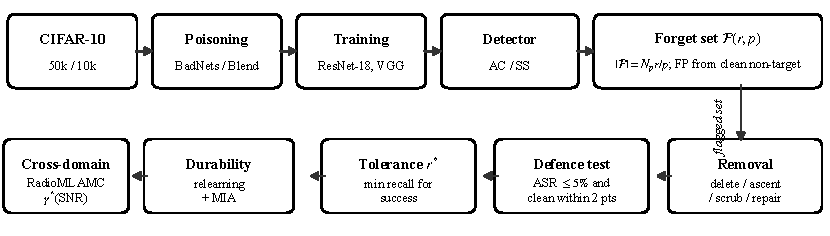
\includegraphics[width=\textwidth]{fig1_pipeline.pdf}
\caption{The measurement pipeline. A poisoned training set yields a backdoored
model, a detector flags a subset, and the flagged set is converted into a forget
set $\fset(r,p)$ with controlled recall and precision. Removal is then scored on
attack success and clean accuracy, summarised as the tolerance $\rstar$,
probed for durability under relearning, and repeated on a radio-modulation
task.}
\label{fig:pipeline}
\end{figure*}

\section{Related Work}
\label{sec:related}

\subsection{Backdoor Attacks}
Backdoor poisoning was established by Gu \etal{} with BadNets, a small
checkerboard patch stamped onto a fraction of training images and relabelled to a
target class \cite{badnets}. Liu \etal{} showed that the same effect can be
obtained by perturbing weights rather than data \cite{trojannn}, and Chen \etal{}
gave an early data-poisoning formulation with a learned trigger
\cite{blendattack}. Later work made the trigger stealthier: clean-label attacks
that require no label change \cite{cleanlabel}, hidden-trigger attacks that
optimise the poisoned input to be far from the trigger at test time
\cite{hidden}, warping-based triggers \cite{wanet}, learnable and imperceptible
triggers \cite{lira}, input-aware triggers \cite{inputaware}, and physically
realisable triggers \cite{physical}. In federated learning, a single malicious
client can inject a backdoor that survives aggregation
\cite{bagdasaryan,bhagoji,dba}. Surveys by Li \etal{} \cite{survey} and Goldblum
\etal{} \cite{goldblum} organise this space and stress that defence evaluation
is fragmented.

Backdoor poisoning is a special case of data poisoning, which has a longer
history: support-vector poisoning \cite{biggio}, certified defences against
poisoning \cite{steinhardt_cert}, poisoning of regression learning
\cite{jagielski}, and attacks that break data sanitization at scale
\cite{kohpoison}, including gradient-matching poisons that transfer across
models \cite{witchesbrew}. The lesson of that line of work, that a defence tuned
to one poisoning strength can fail at another, motivates the sweep over recall
and precision here.

The design space has since widened well beyond dirty-label patches: clean-label
poisoning of feature extractors \cite{poisonfrogs}, subpopulation poisoning
\cite{subpop}, frequency-domain triggers \cite{freq}, reflection triggers
\cite{reflection}, dynamic triggers \cite{dynamic}, and latent backdoors
\cite{latent}; contrastive encoders \cite{carlinicl}; and instruction-tuned
language models \cite{poisonllm}. Data-sanitization defences can themselves be
evaded by stronger poisoning \cite{kohpoison}, and BackdoorBench consolidates
implementations and evaluation protocols across this space
\cite{backdoorbench}.

Our threat model is the simplest and most studied one: an attacker controls a
fraction of a static training set and stamps a fixed, visible trigger. We use two
instances, a $4\times4$ checkerboard and a blended pattern, precisely because
they are canonical. The contribution of this paper is not a new attack but the
measurement of what happens after one is detected imperfectly.

\subsection{Detection}
Detection methods score inputs, features, or model parameters. Neural Cleanse
optimises a minimal trigger per class and flags a class whose trigger is
anomalously small \cite{nc}. ABS stimulates neurons and observes whether a
single output class dominates \cite{abs}. STRIP perturbs inputs with
superimposed patterns and measures prediction entropy \cite{strip}. Activation
clustering projects per-class activations and separates them into two clusters
\cite{ac}, and spectral signatures analyses the top singular direction of
per-class representations \cite{ss}. Fine-pruning observes that backdoored
neurons are dormant on clean inputs and prunes them \cite{finepruning}.
Post-training scanners continue to broaden coverage; MM-BD, for example, scores
classes by a maximum-margin statistic and does not assume a patch-shaped
trigger \cite{mmbd}.

All of these methods trade missed detections against false positives, and their
operating points depend on poison rate, architecture, and attack. Detection is
therefore not a preprocessing detail that can be assumed away: it defines the
input to the removal stage. Recent defences continue to improve the detector
side, including variational formulations that jointly model trigger and
class-conditional structure \cite{seal}. Our study is complementary: we take
detector output as given and ask how much of its error the removal stage can
absorb. To keep the manipulation interpretable we parameterise that output by
recall and precision rather than by a detector-specific threshold, and we anchor
the parameterisation to two real detectors in Section~\ref{sec:cliff}.

\subsection{Removal and Unlearning}
The gold standard for removal is retraining on the retained data
\cite{badnets,finepruning}. Because full retraining is expensive, a large
literature approximates it. SISA shards the training set, trains a constituent
model per shard, and unlearns by retraining only the affected shards
\cite{sisa}. Amnesiac unlearns by ascending the loss on the forget set
\cite{amnesiac}, Eternal Sunshine approximates the retrained weights in a
quadratic Fisher sense \cite{eternal}, and certified removal provides a
differential-privacy-style guarantee for convex or strongly convex models
\cite{certified}. SCRUB trains a student to match the teacher on the retain set
while disagreeing on the forget set \cite{scrub}. Influence functions and
gradient tracing estimate which training points mattered and can be used to
down-weight them \cite{influence,tracin}, and example-forgetting scores have been
proposed as a way to choose which points a model should forget \cite{toneva}.
Suriyakumar and Wilson characterise
the limits of approximate-removal guarantees \cite{limits}. Surveys of machine
unlearning \cite{unlearnsurvey} and domain-specific benchmarks
\cite{tofu,wmdp} have grown around this literature, and what an unlearning claim
should certify is now a central question for language models
\cite{unlearnllm}.

A parallel family acts during or immediately after training rather than on a
forget set: anti-backdoor learning separates poison from clean data while
training \cite{abl}, decoupled training withholds the trigger association from
the feature extractor \cite{decouple}, adversarial neuron pruning removes
trigger-sensitive units \cite{anp}, and attention distillation fine-tunes the
backdoored model on clean data \cite{nad}. Trigger-reverse-engineering scanners
reconstruct a candidate trigger before removal \cite{tabor}. These methods
reduce the need for an exact forget set, but each still needs either clean data,
a clean reference model, or a reconstructed trigger; none is evaluated under a
forget set whose recall is known to be below one.

Closest to our recipe are methods that edit the association rather than delete
the data. Zhao and Wressnegger study the symmetry between learning a backdoor
and removing one \cite{twosides}. Repair-based pipelines relabel flagged samples
and fine-tune, optionally with an inoculation step that presents the trigger
with its correct label. These methods are attractive under imperfect detection
because they do not require the forget set to be exact, but their inoculation
step needs the trigger. We quantify both sides of that trade: the tolerance the
recipe buys, and the knowledge it consumes.

Two 2025 results shape our interpretation. Pawelczyk \etal{} show that
approximate unlearning methods, including methods designed for large language
models, fail to remove the effect of poisoned data even when they appear to
succeed on standard unlearning metrics \cite{pawelczyk}. Hu \etal{} show that
benign relearning restores supposedly unlearned behaviour \cite{jogging}, and
the same persistence under benign retraining has been observed in language
models trained to exhibit deceptive behaviour \cite{sleeper}. Our
durability study is a vision-domain analogue of the second result, and our
overall conclusion is consistent with the first: unlearning metrics that do not
probe the attack after removal can be misleading.

\subsection{Evaluation Under Imperfect Detection}
The gap we address is evaluative. Removal papers usually construct the forget
set from ground-truth poison labels, or from a detector threshold that is tuned
until recall is perfect. Detector papers report recall and precision but stop
before removal. Studies that connect the two usually vary a single threshold and
report a single operating point, which makes it hard to separate the effect of
missed poison from the effect of deleted clean data. Controlled manipulation of
both quantities, across method families and across domains, is what our grid
provides. The tolerance $\rstar$ is intended as a reusable summary: it answers
``how good must the detector be for this removal method to work?'' in the same
units for every method.

\subsection{Calibration and Risk Control}
Calibrate-then-Remove, one of the two refinements we test, borrows the logic of
distribution-free risk control. Conformal prediction converts a score into a
prediction set with a user-specified coverage guarantee under exchangeability
\cite{vovk,angelopoulos}, and conformal risk control extends the guarantee from
coverage to an arbitrary bounded loss \cite{crc}. The same machinery can in
principle choose a removal threshold that controls the risk of a live backdoor. The
guarantee depends on a proxy that is exchangeable with the test trigger. Our
experiment tests whether a synthesised trigger can serve as that proxy; the
answer, on both attacks, is no.

\subsection{Positioning}
This paper is a measurement study with one attempted mechanism and an explicit
negative result. It does not claim a new attack, a new detector, or a deployable
defence. Its contributions are the controlled forget-set construction, the
recall cliff and its transfer across architectures and attacks, the tolerance
metric $\rstar$, the demonstration that trigger synthesis breaks the only method
that tolerates imperfect recall, and the replication of the cliff in a radio
modulation task. The repair recipe we study is a strong baseline and an upper
bound; we label it as such wherever it appears.

\section{Problem Formulation and Metrics}
\label{sec:problem}

\subsection{Setup}
Let $\mathcal{D}=\{(x_i,y_i)\}_{i=1}^{N}$ be a training set and let
$\mathcal{P}\subset\mathcal{D}$ be the poisoned subset, $|\mathcal{P}|=N_p$.
A model $f=\mathcal{A}(\mathcal{D})$ is produced by a fixed training algorithm
$\mathcal{A}$; in this paper $\mathcal{A}$ is the schedule of
Table~\ref{tab:protocol}. For a target class $y_t$ and a trigger function $T$,
the attack success rate is
\begin{equation}
\ASR(f)=\frac{1}{|\mathcal{D}_{\mathrm{test}}|}
\sum_{(x,y)\in\mathcal{D}_{\mathrm{test}}}
\mathbb{1}\!\left[f(T(x))=y_t\right],
\label{eq:asr}
\end{equation}
and clean accuracy is the usual top-1 accuracy on unmodified test inputs. A
backdoor is considered present when $\ASR$ is high and clean accuracy is close
to that of a model trained without poison. The gold reference is
$f_{\mathrm{gold}}=\mathcal{A}(\mathcal{D}\setminus\mathcal{P})$, trained on the
same data with the true poison removed. All success statements are relative to
$f_{\mathrm{gold}}$, not to the poisoned model, because the poisoned model's
clean accuracy can be slightly higher or lower by chance and would otherwise
make weak methods look adequate.

\subsection{Detectors and Their Operating Points}
A detector is a map $\mathrm{DET}:\mathcal{D}\to 2^{\mathcal{D}}$ producing a
flagged set $S$. Relative to the ground-truth poison,
\begin{equation}
r=\frac{|S\cap\mathcal{P}|}{|\mathcal{P}|},\qquad
p=\frac{|S\cap\mathcal{P}|}{|S|},
\label{eq:det}
\end{equation}
with $p$ defined as zero when $S=\emptyset$. Recall $r$ is the fraction of
poison the removal method will see; precision $p$ is the fraction of the flagged
set that is genuinely poisoned. Both matter, but they enter the removal problem
asymmetrically: a missed poison sample remains in the training set and can
sustain the backdoor, whereas a falsely flagged clean sample is merely removed
from training. The experiments are designed to expose that asymmetry.

\subsection{Controlled Forget Sets}
Rather than threshold a detector score, we construct the forget set directly.
For requested recall $r\in[0,1]$ and precision $p\in(0,1]$, let
\begin{equation}
\fset(r,p)=A\cup B,\quad
A\subseteq\mathcal{P},\ |A|=\mathrm{round}(N_p r),
\label{eq:forgetA}
\end{equation}
\begin{equation}
B\subseteq\mathcal{D}_{\mathrm{clean}}\setminus
\mathcal{C}_{y_t},\quad
|B|=\mathrm{round}\!\left(\frac{N_p r(1-p)}{p}\right),
\label{eq:forgetB}
\end{equation}
where $\mathcal{C}_{y_t}$ is the set of clean training samples of the target
class. The sizes follow from the definition of precision: if $|A|=N_p r$ and
$|A|/|A\cup B|=p$, then $|\fset|=N_pr/p$ and $|B|=N_pr(1-p)/p$. False positives
are drawn from non-target clean data so that the forget set never removes clean
examples of the class the attacker wants to protect, which would confound
removal with class deletion. Both $A$ and $B$ are sampled without replacement
with a seed derived from $(r,p,\text{seed})$, so the construction is
deterministic and reproducible. Algorithm~\ref{alg:forget} states the procedure.

\begin{algorithm}[t]
\caption{Controlled forget-set construction}
\label{alg:forget}
\begin{algorithmic}[1]
\Require training set $\mathcal{D}$, poison mask, $r$, $p$, seed $s$
\Ensure $\fset(r,p)$ with $|\fset|=N_pr/p$
\State $\mathcal{P}\gets$ poisoned indices; $N_p\gets|\mathcal{P}|$
\State $n_A\gets\mathrm{round}(N_pr)$
\State $n_B\gets\mathrm{round}(N_pr(1-p)/p)$
\State $A\gets$ sample $n_A$ indices from $\mathcal{P}$ with seed $s$
\State $C\gets$ clean, non-target training indices
\State $B\gets$ sample $n_B$ indices from $C$ with seed $s$
\State \Return $A\cup B$
\end{algorithmic}
\end{algorithm}

The construction has three properties that matter for interpretation. First,
$|\fset|$ grows as $p$ falls at fixed $r$: with $N_p=2{,}500$, the cell
$(r,p)=(0.90,1.0)$ removes 2{,}250 samples, while $(0.90,0.7)$ removes 3{,}214.
Precision is therefore also a measure of how much clean data the method must
give up. Second, $r$ and $p$ are requested values; the realised values are stored
with each run and differ only by rounding, because the counts are integers.
Third, the construction is deliberately kinder than a real detector in one
respect: it never places a false positive in the target class and it never
places poison in the retain set when $r=1$. Real detectors do both. The grid is
therefore a best-case controlled manipulation of detector error, not a
simulation of a specific detector. Section~\ref{sec:cliff} anchors it to two real
detectors by running the same removal methods on their raw flag sets.

\subsection{Defence Success and the Tolerance $\rstar$}
A removal run is a success when both halves of the following criterion hold:
\begin{equation}
\ASR(f')\leq 5\%\quad\text{and}\quad
\mathrm{Acc}_{\mathrm{clean}}(f')\geq
\mathrm{Acc}_{\mathrm{clean}}(f_{\mathrm{gold}})-2.
\label{eq:success}
\end{equation}
The first half says the backdoor is no longer usable at a rate that would matter
to an attacker; the second says the cure did not cost more than two points of
utility. The two-point budget is a modelling choice; it is wide enough to absorb
seed noise (the gold model itself varies by about $\pm0.1$ points) and narrow
enough to exclude methods that remove the backdoor by damaging the network. We
report the two quantities separately in every table so that a reader who prefers
a different budget can re-derive the verdicts. For each method we then define
\begin{equation}
\begin{aligned}
\rstar=\min\Bigl\{r:\ &\overline{\ASR}(r,1)\leq 5\%\ \text{and}\\
&\overline{\mathrm{Acc}}_{\mathrm{clean}}(r,1)\geq
\overline{\mathrm{Acc}}_{\mathrm{clean}}(f_{\mathrm{gold}})-2\Bigr\},
\end{aligned}
\label{eq:rstar}
\end{equation}
where the bar is the mean over the three seeds, and write $\rstar=\text{--}$ when
no recall in the grid succeeds. We use the mean because the criterion describes a
deployment, not a single training run; the per-seed counts are reported
separately in Table~\ref{tab:success} so that a reader who requires unanimity can
see exactly where the two readings diverge. The tolerance is a property of a
removal method, not of a detector: it states how much detector recall the method
needs before it can be relied on.

\subsection{Secondary Metrics}
For the amplification study we ask whether partial removal makes missed poison
separable from clean data. Let $\mathcal{M}=\mathcal{P}\setminus\fset$ be the
poison missed by the forget set and let $\mathcal{C}_0$ be clean
training data of the target class. We fit a detector score to distinguish
$\mathcal{M}$ from $\mathcal{C}_0$ and report the area under the ROC curve,
\begin{equation}
\mathrm{AUC}=\Pr\!\left[s(x_{\mathrm{missed}})>s(x_{\mathrm{clean}})\right],
\label{eq:auc}
\end{equation}
with ties counted at one half. An AUC of 0.5 is chance. For durability we report
ASR after $k$ gradient steps on fresh poison, a loss-threshold membership
inference AUC following Shokri \etal{} \cite{mia}, and the Kullback--Leibler
divergence between the output distributions on clean and trigger-stamped inputs.
A live backdoor shows a large clean-versus-trigger divergence; a dormant one does
not.

\subsection{Statistical Treatment}
Every CIFAR-10 cell is run with seeds 0, 1, and 2. Poison placement, weight
initialisation, and data order vary with the seed; the training and test splits
do not. We report mean $\pm$ standard deviation over seeds and, for the success
criterion, the count of seeds that pass. With three seeds the counts are coarse,
and we do not attach confidence intervals to them. When a method is bimodal
across seeds (NegGrad+ is the clearest case), the mean and standard deviation
describe a mixture rather than a stable operating point; we say so in the table
notes instead of hiding it in a single number.

\section{Removal Methods and Detector Models}
\label{sec:methods}

All removal methods start from the poisoned model $f$ except the two retraining
methods, which start from random initialisation. The post-training methods use
SGD with momentum 0.9 and weight decay $5\times10^{-4}$, and are deliberately
kept simple: the goal is to compare families under a common budget, not to tune
each family to its best. The CIFAR-10 settings common to all runs are listed in
Table~\ref{tab:protocol}.

\subsection{Deletion and Retraining}
\method{Retrain}$_{\setminus F}$ is the reference deletion method: train a new
network from scratch on $\mathcal{D}\setminus\fset$ with the full twelve-epoch
schedule. It is expensive, but it is the method that the oracle literature
reports as a success, and it isolates the effect of the forget set from any
property of the poisoned initialisation. When $\fset$ equals the true poison
set, this is the gold model.

\subsection{Fine-Tuning on the Retained Set}
\method{Fine-tune} continues training the poisoned model for three epochs at
learning rate $0.01$ on $\mathcal{D}\setminus\fset$. It is the cheapest possible
response to a detector and is common in practice when retraining is not
affordable. It has no mechanism for forgetting: it only reinforces the retained
data.

\subsection{Gradient Ascent and SCRUB}
\method{NegGrad+} performs three epochs of ascent on the cross-entropy of the
forget set, balanced by descent on a matched random batch from the retained set,
at learning rate $10^{-3}$ \cite{amnesiac}. \method{SCRUB} first fine-tunes a
teacher on the retained set for three epochs, then trains a student for three
epochs to minimise cross-entropy on the retained set plus a Kullback--Leibler
term that pulls the student's distribution on the forget set towards the
teacher's \cite{scrub}. Both methods are designed for exact forget sets; the
grid tests how they behave when the set is noisy.

\subsection{Repair and Inoculation}
The recipe is the only method in the suite that is designed around an imperfect
forget set. It has two stages.

\emph{Label repair.} Features are extracted from the penultimate layer of the
poisoned model for all training samples. Each flagged sample receives a
pseudo-label by a weighted $k$-nearest-neighbour vote ($k{=}10$,
inverse-distance weights) over the \emph{unflagged, non-target} training data.
The sample is kept, not deleted, with its repaired label. The intuition is that
a poisoned image whose patch is ignored looks like its true class, so the
nearest neighbours in feature space are clean images of that class rather than
of the target class.

\emph{Inoculation.} A pool of 5{,}000 retained samples that the poisoned model
does not confidently classify as the target class is trigger-stamped and kept
with its true label. Each mini-batch is composed of 60\% retained samples, 20\%
flagged samples with pseudo-labels, and 20\% inoculated samples. The network is
fine-tuned for three epochs at learning rate $0.01$. Presenting the trigger with
the correct label teaches the network that the trigger is not predictive of the
target class, which is the mechanism by which the recipe can tolerate poison
that the forget set missed. Fig.~\ref{fig:recipe} draws the two streams and where
they meet.

\begin{figure}[t]
\centering
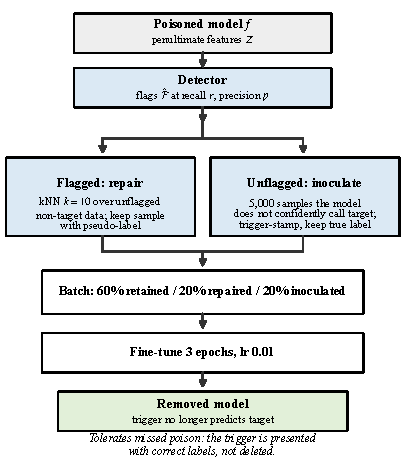
\includegraphics[width=0.92\columnwidth]{fig14_recipe_pipeline.pdf}
\caption{The repair-and-inoculate recipe. Flagged samples are relabelled by a
$k$-nearest-neighbour vote over unflagged, non-target data; unflagged samples
supply the trigger-stamped inoculation pool. The streams are mixed 60/20/20 and
fine-tuned for three epochs. The lower branch is what tolerates missed poison:
the trigger is presented with correct labels rather than deleted.}
\label{fig:recipe}
\end{figure}

\emph{Inoculation only.} To separate the two stages we also run an
inoculation-only variant that keeps the entire training set, applies no label
repair, and fine-tunes with 20\% trigger-stamped samples for three epochs. This
is the F-independent baseline of the E1 grid: it uses no forget set at all and
therefore cannot degrade with detector recall, but it also cannot repair the
poisoned labels. A second variant replaces the true trigger with a synthesised
one (Section~\ref{sec:general}).

\subsection{Trigger Synthesis}
The synthesis baseline follows Neural Cleanse \cite{nc}. For each class other
than the target, a soft mask $m\in[0,1]^{32\times32}$ and a pattern are optimised
for 200 Adam steps at learning rate $0.1$ on 64 samples of that class, with the
objective of driving the model to the target class while penalising the mask
mass with weight $10^{-3}$. The class with the smallest mask mass is retained as
the estimated trigger. The overlap with the true patch is measured by
intersection over union (IoU) after thresholding the mask at $0.5$. The
synthesised trigger is then used wherever the true trigger would be used, both
for inoculation and as the proxy in Calibrate-then-Remove.

\subsection{Calibrate-then-Remove}
Calibrate-then-Remove (CaR) is our attempted mechanism for turning detector
output into a removal decision with a guarantee. For a grid of spectral-signature
thresholds $\theta$, it forms the corresponding forget set, applies the recipe's
repair stage to obtain a proxy-removed model, and measures the proxy model's
response $\tau$ to the \emph{synthesised} trigger. If a threshold yields
$\tau\leq5\%$, the same threshold is applied to the real test trigger and the
removal is accepted. If no threshold qualifies, the method falls back to the
F1-optimal threshold. The logic is conformal in spirit: the synthesised trigger
plays the role of a calibration sample that is exchangeable with the test
trigger \cite{vovk,angelopoulos}. It fails if the synthesised trigger is not a
valid proxy, which is what we observe.

\subsection{Amplify-and-Detect}
The second attempted mechanism tests a hypothesis rather than a pipeline: that
partial unlearning makes the poison it failed to remove easier to detect, because
the network must reallocate the trigger association onto the residual poison and
therefore represents it more sharply. We operationalise it by applying partial
label repair at two strengths, then fitting a detector to separate the missed
poison from clean target-class data and measuring AUC \eqref{eq:auc}. The
pre-registered promotion gate required an AUC gain of at least $+0.10$ over the
base model, a clean-accuracy loss of at most two points, and a gain larger than a
matched clean-removal control that receives the same intervention on clean data
instead of poison. All three clauses had to hold on all seeds.

\subsection{Detectors}
We use two published detectors, both applied to the penultimate features of the
poisoned model.

\emph{Activation clustering} \cite{ac} processes each class separately: it
projects the class's features to ten principal components, runs $k$-means with
$k{=}2$, and flags the smaller cluster if its size fraction is below 0.35 and
the silhouette score exceeds 0.10.

\emph{Spectral signatures} \cite{ss} computes, for each class, the top singular
vector of the centred feature matrix and scores every sample by the squared
projection onto that direction. It flags a fixed budget of $1.5N_p$ samples with
the largest scores. The fixed budget is why its precision degrades at low poison
rates: at a 1\% poison rate the budget is 750 samples for 500 true poison, and at
5\% it is 3{,}750 for 2{,}500.

Fig.~\ref{fig:detpipeline} draws the two pipelines side by side. Both read the
same penultimate features and differ only in how they score a sample; the two
annotations mark the failure modes that recur in the grid, an empty flag set at
10\% poison for activation clustering and a 33.8\% recall at 1\% for spectral
signatures.

\begin{figure*}[t]
\centering
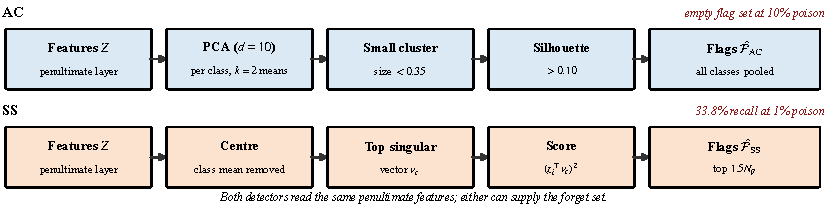
\includegraphics[width=\textwidth]{fig12_detection_pipeline.pdf}
\caption{The two detectors as pipelines. Both read the same penultimate
features. Activation clustering (top) returns no flags at a 10\% poison rate;
spectral signatures (bottom) recovers 33.8\% of the poison at a 1\% rate because
its fixed $1.5N_p$ budget lets clean samples crowd out poison.}
\label{fig:detpipeline}
\end{figure*}

Both detectors were also run on VGG-16-BN and MobileNetV2 models. Those runs were
degenerate (no flags, or flags with no true positives) and are excluded from the
tables; we report the ResNet-18 operating points, which are the ones that
produce non-trivial forget sets.

\subsection{Efficiency-Oriented Baselines}
Two further baselines are included for completeness. SISA-5 shards the training
set into five parts, trains one model per shard, and unlearns by retraining the
shards that contain forget-set samples \cite{sisa}; we report both the
oracle-recall variant and a recall-0.5 variant. Fine-pruning removes filters
with the smallest average activation on clean data, in increasing fractions
\cite{finepruning}. These methods are not swept over the grid because their
compute profile is different, but they answer the natural question of whether a
cheaper mechanism can substitute for deletion.

\subsection{What Each Family Needs}
Fig.~\ref{fig:families} arranges the families by what they consume. Deletion is
the only method that never touches the poisoned weights; it discards the network
and pays a full schedule. Fine-tuning and the two ascent methods all start from
the poisoned model and differ only in how they use $\fset$, and all three assume
that $\fset$ is the poison, which is the assumption the grid relaxes. The recipe
is the only family that consumes the trigger, and that is the asymmetry the
figure is meant to make visible: trigger knowledge buys tolerance to an
incomplete $\fset$, and nothing else in the suite has it. The compute column
also explains why the efficiency-oriented methods are evaluated separately
rather than inside the grid: deletion buys its clean removal with a full
schedule, while the three-epoch methods are cheap precisely because they stay
close to the poisoned model.

\begin{figure*}[t]
\centering
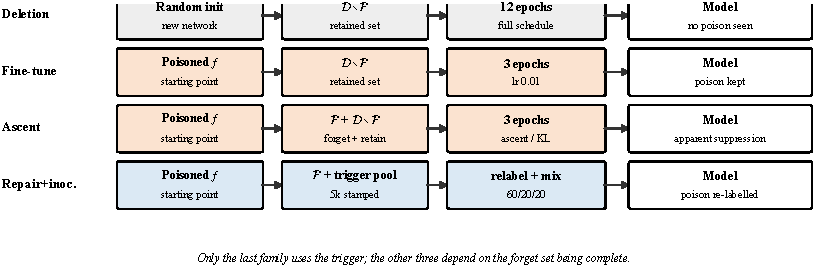
\includegraphics[width=\textwidth]{fig13_removal_families.pdf}
\caption{The four removal families and what each consumes. Only the
repair-and-inoculation family uses the trigger; the other three assume that the
forget set is the poison. The last column states the intended mechanism, not the
measured outcome.}
\label{fig:families}
\end{figure*}

\section{Experimental Protocol}
\label{sec:protocol}

\subsection{CIFAR-10}
We use CIFAR-10 \cite{cifar}: 50{,}000 training and 10{,}000 test images of
$32\times32$ pixels in ten classes, with class 0 as the attack target. Poisoning
is dirty-label: a fraction of non-target training images receive the trigger and
their labels are set to the target. BadNets stamps a $4\times4$ checkerboard of
alternating 1/0 pixels on rows and columns 27--30 \cite{badnets}. Blend replaces
the image by
$0.8x+0.2\pi$, where $\pi$ is a fixed uniform pattern generated with seed 123
\cite{blendattack}. The poison rate is 5\% (2{,}500 samples) except in the
amplification study, which uses 10\% (5{,}000 samples) to give the detector more
signal.

We train CIFAR variants of ResNet-18 \cite{resnet} and VGG-16-BN \cite{vgg} for
12 epochs with SGD (Nesterov momentum 0.9, weight decay
$5\times10^{-4}$), a OneCycle schedule with maximum learning rate 0.1 (0.05 for
VGG), batch size 512, random crop to $28\times28$ with padding 4, horizontal
flip, and mixed precision \cite{onecycle,bn,pytorch}. Normalisation is applied
inside the model. Three seeds (0, 1, 2) vary poison placement, initialisation,
and data order; the train/test split is fixed. Each seed therefore yields its own
gold model, and success is always judged against that seed's gold accuracy
($88.59$, $88.65$, and $88.77\%$ for seeds 0--2 respectively). The total CIFAR
compute was approximately 23 GPU-hours on two T4 cards.

Attack success is measured on the non-target test images after stamping the
trigger, so a model that predicts the target class indiscriminately cannot score
well by accident. Clean accuracy is measured on the unmodified test set.

\subsection{RadioML Automatic Modulation Classification}
The cross-domain study uses RadioML 2016.10a \cite{radioml,radioml_jstsp}: eleven
modulation classes, SNR from $-20$ to $18$\,dB in 2\,dB steps, each sample a
$2\times128$ in-phase/quadrature window. Samples are normalised to unit energy.
The classifier is a three-block one-dimensional CNN (32, 64, and 128 channels,
batch normalisation, max pooling, global average pooling) trained for 12 epochs
with Adam at learning rate $10^{-3}$ and weight decay $10^{-4}$. The trigger is
a fixed burst that sets $I{=}0.9$ and $Q{=}{-}0.9$ on the last eight samples,
and 5\% of the non-target training windows are stamped and relabelled to BPSK.
The split is 80/20 and fixed across seeds; poison placement and initialisation
vary. Removal methods are fine-tuned for four epochs at learning rate $10^{-4}$.
Four methods (gold retrain, retain fine-tuning, recipe, and inoculation-only) are
run at recall 1.0, 0.75, and 0.5 with precision 1.0, plus a precision-0.7 cell at
recall 0.75. Attack success and clean accuracy are evaluated per SNR bin.

We emphasise one protocol detail because it changes how the results must be read.
At SNR below about $-12$\,dB the clean classifier is close to chance (9.1\% for
eleven balanced classes), and an ASR threshold of 5\% is then not a
meaningful test of a defence: even the oracle retrain sits above it. We therefore
report $\gstar$ for every SNR but mark the near-chance region and restrict
interpretation to SNR at or above $-6$\,dB, where clean accuracy is at least
48\%.

\subsection{What Is Frozen}
The four experiment drivers were frozen before the final runs and were not
edited afterwards. Each driver writes one CSV row per run, including the
requested and realised recall and precision, the forget-set size, clean
accuracy, ASR, wall-clock time, and free-text notes. All figures and tables in
this paper are generated from those rows by a single analysis script; no
number was transcribed by hand. Where a run produced a degenerate detector
output (no flags, or flags containing no true poison) the row is kept in the
records and excluded from the corresponding table with a note. The logs are keyed
by person, experiment, architecture, attack, poison rate, seed, requested recall
and precision, method, and detector, so any table can be reconstructed by
filtering the logs; the analysis script applies those filters and writes the
\LaTeX{} tables and the PDF figures directly. Fig.~\ref{fig:arch} traces the
chain from the frozen core to the compiled PDF; because the analysis is a
deterministic function of the CSVs, every table can be regenerated without
rerunning a model.

\begin{figure*}[t]
\centering
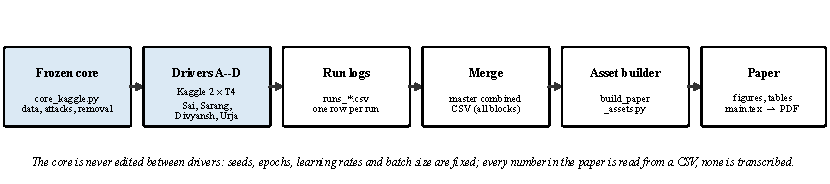
\includegraphics[width=\textwidth]{fig15_code_arch.pdf}
\caption{The artifact chain. Four frozen drivers write one CSV row per run, the
rows are merged into a master table, and the asset builder reads that table to
write the \LaTeX{} tables and PDF figures in this paper. No number is typed by
hand.}
\label{fig:arch}
\end{figure*}

\begin{table}[t]
\centering
\caption{Frozen experimental protocol. Every row of every table in this paper was produced under these settings; only the listed knobs vary between experiments.}
\label{tab:protocol}
\footnotesize
\begin{tabular}{@{}l >{\raggedright\arraybackslash}p{0.64\columnwidth}@{}}
\toprule
\textbf{Item} & \textbf{Setting} \\
\midrule
Dataset & CIFAR-10, 50k train / 10k test, 10 classes, target class 0 \\
Attacks & BadNets $4\times4$ checkerboard (rows/cols 27--30); Blend $0.8x+0.2\,\mathrm{pattern}$, seed 123 \\
Poison rate & 5\% (2{,}500 samples); 10\% in the amplification study \\
Architectures & ResNet-18, VGG-16-BN (CIFAR variants) \\
Optimiser & SGD, momentum 0.9 (Nesterov), weight decay $5\times10^{-4}$ \\
Schedule & OneCycleLR, max lr 0.1 (VGG 0.05), 12 epochs, batch 512 \\
Augmentation & random crop 32$\to$28 with padding 4, horizontal flip; normalisation inside the model \\
Seeds & 0, 1, 2 (identical splits; poison placement and init vary) \\
Detectors & Activation Clustering; Spectral Signatures (per-class, PCA/2-means resp.\ top singular vector) \\
Forget set & $\mathcal{F}(r,p)$: $N_p r$ true poison $+$ $N_p r(1-p)/p$ clean non-target false positives \\
Defence success & ASR $\leq5\%$ \emph{and} clean accuracy within 2 points of the gold retrain \\
Hardware & Kaggle 2$\times$T4 (16 GB each), mixed precision; $\approx$23 GPU-hours total \\
\bottomrule
\end{tabular}
\end{table}


\begin{table}[t]
\centering
\caption{Experiment blocks. E4 was planned and not executed; every other block is
reported in the section listed.}
\label{tab:blocks}
\footnotesize
\setlength{\tabcolsep}{3.5pt}
\begin{tabular}{@{}l >{\raggedright\arraybackslash}p{0.30\columnwidth} >{\raggedright\arraybackslash}p{0.34\columnwidth} c@{}}
\toprule
\textbf{Block} & \textbf{Question} & \textbf{What was run} & \textbf{Sec.} \\
\midrule
E1 & Does removal survive imperfect recall? & 10 $(r,p)$ cells $\times$ 5 methods $\times$ 3 seeds, ResNet-18/BadNets; inoculation-only baseline & VI \\
E2 & Is the cliff about residual poison? & 4 architecture--attack pairs $\times$ 5 residual fractions (0--100\%) & VI \\
E3 & Can calibration choose the threshold? & 20 SS thresholds with proxy removal; two full retrains & VIII \\
E4 & Does an adaptive attacker break the recipe? & planned, not executed & XII \\
E5 & Erasure or suppression? & 4 settings $\times$ relearning to 50 steps; MIA and KL probes & IX \\
E6 & Do real detector columns reproduce the cliff? & AC and SS at 1\%, 5\%, 10\% poison; deletion and recipe at realised operating points & VI \\
E7 & Does the cliff transfer? & VGG-16-BN/BadNets, VGG-16-BN/Blend, ResNet-18/Blend at $r{=}0.75,0.5$ & VII \\
E7b & Can the trigger be synthesised? & Neural-Cleanse synthesis on two attacks & VII \\
E8 & Is ascent removal real? & 4 ascent strengths $\times$ raw and BN-guarded & VIII \\
E9 & Does partial repair amplify detectability? & 10\% poison, 3 seeds $\times$ 2 repair strengths $+$ matched controls & VIII \\
SISA & How do efficiency-oriented baselines compare? & SISA-5 shards; fine-pruning at two thresholds & IX \\
RF & Does the cliff cross domains? & RadioML AMC, 4 methods $\times$ 3 recalls, 20 SNR bins, 3 seeds & X \\
\bottomrule
\end{tabular}
\end{table}


\subsection{Scope of the Evidence}
Table~\ref{tab:blocks} lists the experiment blocks, what each was run for, and
where it is reported. The CIFAR grid covers two architectures, two attacks,
three seeds, five removal families, and ten recall--precision cells; the
amplification study adds a third detector operating point at 10\% poison. The radio study covers one architecture,
one attack, three seeds, four methods, and twenty SNR bins. Two blocks that were
planned in the protocol were not executed: an adaptive-attacker study (E4) and a
full hyperparameter sweep for the baselines. We state this explicitly in
Section~\ref{sec:limits} rather than implying coverage we do not have. The claims
in this paper are correspondingly bounded: they concern post-training removal
under the stated attacks and budgets, not the impossibility of defence in
general.

\section{The Recall Cliff}
\label{sec:cliff}

\subsection{Detector Operating Points}
Table~\ref{tab:detector} and Fig.~\ref{fig:detector} report the two detectors on
ResNet-18/BadNets models at poison rates of 1\%, 5\%, and 10\%. Three features of
these measurements motivate the rest of the paper.

First, recall is not free. Spectral signatures flags a fixed budget of $1.5N_p$
samples and recovers only 33.8\% of the poison at a 1\% poison rate, because the
top-scoring clean samples crowd out poison at that scale. Activation clustering
recovers all of it at 1\% and 5\%, but at 10\% it returns an empty flag set: the
class-0 cluster no longer passes its size and silhouette tests, so the detector
reports that nothing is wrong at exactly the poison rate where the attack is
strongest.

Second, precision degrades as recall improves. At 5\%, activation clustering
flags 4{,}140 samples for 2{,}500 true poison (precision 0.60) and spectral
signatures flags 3{,}750 (precision 0.64). A removal method therefore receives a
forget set in which roughly one third of the entries are clean images.

Third, architecture matters. The same detectors on VGG-16-BN and MobileNetV2
produced degenerate outputs (no flags, or flags with no true positives) and are
excluded. Detector behaviour is not a property of the attack alone; it is a
property of the representation, which is why a controlled parameterisation of
detector output is more portable than a fixed threshold.

\begin{table}[t]
\centering
\caption{Measured detector operating points: the noisy forget sets that motivate the grid.}
\label{tab:detector}
\footnotesize
\begin{tabular}{cccccc}
\toprule
\textbf{Poison} & \textbf{Det.} & \textbf{Flagged} & \textbf{TP} & \textbf{Precision} & \textbf{Recall} \\
\midrule
1\% & AC & 507 & 500 & 0.986 & 1.000 \\
1\% & SS & 750 & 169 & 0.225 & 0.338 \\
5\% & AC & 4,140 & 2,500 & 0.604 & 1.000 \\
5\% & SS & 3,750 & 2,411 & 0.643 & 0.965 \\
10\% & AC & 0 & 0 & -- & -- \\
10\% & SS & 7,500 & 2,400 & 0.320 & 0.480 \\
\bottomrule
\end{tabular}
\par\vspace{1pt}\footnotesize\raggedright Detector output on a ResNet-18/BadNets model; TP is the number of true poison samples among the flags. At 10\% poison, AC returns an empty flag set (no cluster passes its size/silhouette test), i.e.\ $r=0$: the detector, not the removal method, is the binding constraint. VGG-16-BN and MobileNetV2 detector runs were degenerate (no flags or no true positives) and are excluded.
\end{table}


\begin{figure}[t]
\centering
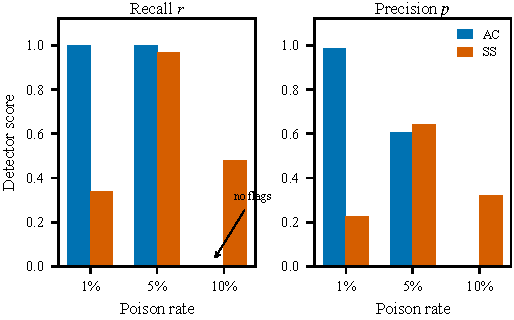
\includegraphics[width=\columnwidth]{fig10_detector.pdf}
\caption{Detector recall and precision on ResNet-18/BadNets at three poison
rates. Activation clustering (AC) returns no flags at 10\% poison; spectral
signatures (SS) is limited by its fixed $1.5N_p$ flag budget at 1\%.}
\label{fig:detector}
\end{figure}

\subsection{Deletion Collapses Between $r{=}0.95$ and $r{=}0.90$}
Fig.~\ref{fig:cliff} and Table~\ref{tab:e1grid} give the central result.
Retraining on the retained set is essentially perfect when the forget set
contains every poisoned sample: ASR $1.68\pm0.26\%$ at $r{=}1$, with clean
accuracy $88.67\%$ against a gold value of $88.59$--$88.77\%$. It remains low at
$r{=}0.95$ (ASR $2.84\pm0.73\%$), but the clean accuracy of that model is
$84.58\%$, four points below gold, so the joint criterion already fails. At
$r{=}0.90$ the backdoor is fully back: ASR $100.00\pm0.00\%$ with clean
accuracy $88.80\%$. From there down to $r{=}0.25$ the ASR stays between 99.63
and 100.00\%. The transition is not gradual. Removing 2{,}375 of 2{,}500 poison
samples leaves a model that still cannot be attacked at a useful rate; removing
2{,}250 does not.

The $r{=}0.95$ cell deserves a comment because it looks like a counterexample.
No clean samples are removed there ($p{=}1$), so the four-point clean-accuracy
drop cannot be a false-positive effect. It is a property of retraining on a set
that still contains 125 poison samples, and we did not isolate the mechanism. We
report it as measured; the practical consequence is the same, because the joint
criterion is what a deployment decision would use. It is also the reason
$\rstar{=}1.00$ rather than $0.95$: the ASR cliff is at 0.90, but the success
cliff is at 1.00.

\begin{figure}[t]
\centering
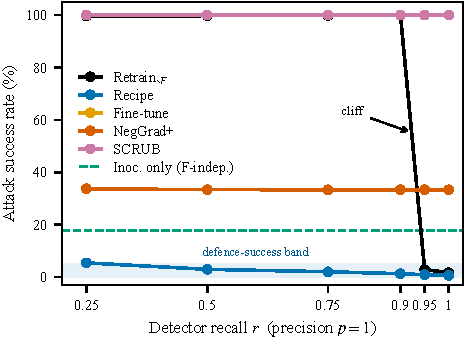
\includegraphics[width=\columnwidth]{fig2_e1_cliff.pdf}
\caption{Attack success after removal as a function of detector recall at
precision 1.0 (mean over three seeds). Deletion is flat at 100\% for
$r\leq0.90$ and drops only when every poisoned sample is removed. The dashed
line is the inoculation-only baseline, which uses no forget set; the shaded band
is the 5\% success threshold.}
\label{fig:cliff}
\end{figure}

\begin{table*}[t]
\centering
\caption{E1: the recall--precision grid. Deletion meets the success criterion only at full recall; repair$+$inoculation holds ASR below 5\% down to $r{=}0.5$.}
\label{tab:e1grid}
\scriptsize
\begin{tabular}{ccrccccc}
\toprule
\textbf{$r$} & \textbf{$p$} & \textbf{$|\mathcal{F}|$} & \textbf{Retrain$_{\setminus F}$} & \textbf{Fine-tune} & \textbf{NegGrad+} & \textbf{SCRUB} & \textbf{Recipe} \\
\midrule
1.00 & 1.0 & 2,500 & \textbf{1.68$\pm$0.26} & 100.00$\pm$0.00 & 33.33$\pm$57.74 & 100.00$\pm$0.00 & \textbf{0.63$\pm$0.21} \\
0.95 & 1.0 & 2,375 & \textbf{2.84$\pm$0.73} & 100.00$\pm$0.00 & 33.33$\pm$57.74 & 100.00$\pm$0.00 & \textbf{0.90$\pm$0.11} \\
0.90 & 1.0 & 2,250 & 100.00$\pm$0.00 & 100.00$\pm$0.00 & 33.33$\pm$57.74 & 100.00$\pm$0.00 & \textbf{1.27$\pm$0.58} \\
0.75 & 1.0 & 1,875 & 99.78$\pm$0.22 & 100.00$\pm$0.01 & 33.33$\pm$57.74 & 100.00$\pm$0.00 & \textbf{2.03$\pm$1.32} \\
0.50 & 1.0 & 1,250 & 99.76$\pm$0.31 & 100.00$\pm$0.01 & 33.35$\pm$57.72 & 100.00$\pm$0.00 & \textbf{2.95$\pm$0.78} \\
0.25 & 1.0 & 625 & 99.63$\pm$0.58 & 99.97$\pm$0.02 & 33.71$\pm$57.41 & 100.00$\pm$0.00 & 5.42$\pm$1.82 \\
0.90 & 0.9 & 2,500 & 99.99$\pm$0.01 & 100.00$\pm$0.00 & 33.33$\pm$57.74 & 100.00$\pm$0.00 & \textbf{1.16$\pm$0.43} \\
0.90 & 0.7 & 3,214 & 99.99$\pm$0.02 & 100.00$\pm$0.00 & 33.33$\pm$57.74 & 100.00$\pm$0.00 & \textbf{1.90$\pm$0.34} \\
0.50 & 0.9 & 1,389 & 99.77$\pm$0.21 & 99.97$\pm$0.03 & 33.35$\pm$57.72 & 100.00$\pm$0.00 & \textbf{3.57$\pm$0.40} \\
0.50 & 0.7 & 1,786 & 99.90$\pm$0.15 & 99.99$\pm$0.01 & 33.34$\pm$57.73 & 100.00$\pm$0.00 & \textbf{2.59$\pm$1.03} \\
\bottomrule
\end{tabular}
\par\vspace{1pt}\scriptsize\raggedright ASR (\%) after removal, mean$\pm$s.d.\ over three seeds; \textbf{bold} marks mean ASR $\leq5\%$ (the ASR half of defence success; clean accuracy is checked in Table~\ref{tab:success}). $|\mathcal{F}|$ is reported for the seed-0 draw (identical across seeds up to rounding). NegGrad+ is bimodal across seeds: two seeds drive ASR to $\approx  0$ while collapsing clean accuracy to 75--86\% at $p{=}1$ (in the four $p<1$ cells one of those seeds collapses further to 10\%), one stays fully inert (ASR 100\%); the mean and s.d.\ describe the mixture, not a stable operating point.
\end{table*}


\subsection{The Cliff Is a Function of Residual Poison}
A separate block (E2) varies the fraction of poison left in the training set
directly, without a detector and without simulated false positives.
Table~\ref{tab:residual} and Fig.~\ref{fig:residual} show the result for the four
architecture--attack combinations. With 0\%, 25\%, 50\%, or 75\% of the poison
still present, ASR is between 99.83\% and 100.00\% in every cell. At complete
removal it falls to 0.59--1.22\%. Clean accuracy varies by at most 0.9 points
across the five fractions within each setting, so the collapse is not a
side-effect of a damaged network. The shape is a step, and the step is located at
zero residual poison. This is the same phenomenon as the grid's $r{=}1$
boundary, seen from the other side: what matters is not how much poison was
deleted but whether any remains. The absolute clean accuracies in E2 are
89.2--90.5\%, slightly above the E1 gold values, because the block was trained
separately; the ASR pattern, not the absolute accuracy, is the object of
comparison.

\begin{table}[t]
\centering
\caption{E2: the cliff is a step function of residual poison, not of the amount deleted.}
\label{tab:residual}
\footnotesize
\setlength{\tabcolsep}{4.5pt}
\begin{tabular}{lcccccc}
\toprule
\textbf{Setting} & \textbf{0\%} & \textbf{25\%} & \textbf{50\%} & \textbf{75\%} & \textbf{100\%} & \textbf{Gold} \\
\midrule
R18/BadNets & 99.83 & 99.98 & 99.94 & 100.00 & 1.21 & 90.3 \\
R18/Blend & 99.99 & 99.97 & 99.97 & 99.86 & 0.64 & 90.2 \\
VGG/BadNets & 100.00 & 99.99 & 100.00 & 100.00 & 1.22 & 89.7 \\
VGG/Blend & 99.97 & 100.00 & 99.94 & 99.98 & 0.59 & 89.7 \\
\bottomrule
\end{tabular}
\par\vspace{1pt}\footnotesize\raggedright ASR (\%) versus the fraction of poison left in the training set after deletion. The last column is the gold retrain's clean accuracy for that setting; across the five residual fractions, clean accuracy varies by at most 0.9 points in every setting, so the cliff is not an accuracy artefact.
\end{table}


\begin{figure}[t]
\centering
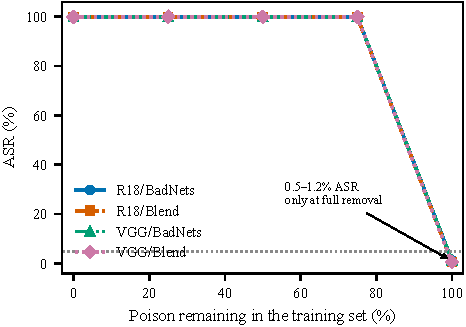
\includegraphics[width=\columnwidth]{fig4_e2_residual.pdf}
\caption{ASR versus the fraction of poison remaining in the training set, for
four architecture--attack combinations. The curve is flat until the poison is
completely gone.}
\label{fig:residual}
\end{figure}

\subsection{Precision Is Secondary to Recall}
The precision axis is much flatter than the recall axis. At fixed $r{=}0.90$,
moving from $p{=}1.0$ to $p{=}0.9$ or $p{=}0.7$ enlarges the forget set from
2{,}250 to 2{,}500 or 3{,}214 samples, and deletion's ASR moves from
$100.00\%$ to $99.99\%$ in both cases. At fixed $r{=}0.50$, $p{=}0.7$ gives
$99.90\%$ against $99.76\%$ at $p{=}1.0$. For the recipe the same manipulation is
visible but small: ASR goes from $1.27\%$ to $1.90\%$ at $r{=}0.9$ and from
$2.95\%$ to $2.59\%$ at $r{=}0.5$, with no consistent direction. Deleting extra
clean data costs some accuracy (the recipe's clean accuracy moves within about
0.6 points), but it neither rescues nor destroys a removal that is otherwise
working.

The asymmetry has a simple reading. A false positive is a clean sample removed
from training, which the network can absorb if the dataset is large. A false
negative is a poisoned sample kept in training, which re-installs the association
the removal was meant to break. At a 5\% poison rate, the largest precision
penalty we test ($p{=}0.7$) adds 714 clean samples to a 50{,}000-sample training
set, a 1.4\% perturbation. The smallest recall penalty we test ($r{=}0.95$)
leaves 125 poison samples, which is enough to matter. Detector engineering for
removal should therefore optimise recall first and treat precision as a budget
constraint.

\subsection{The Other Method Families}
The remaining families do not merely fail at low recall; most of them fail at
full recall as well.

\method{Fine-tune} never removes the backdoor: ASR is $100.00\pm0.00\%$ at
$r{=}1$ and above 99.96\% in every other cell, while clean accuracy is
unaffected ($89.02\%$). Three epochs on the retained set reinforce whatever the
poisoned model already represents.

\method{NegGrad+} is bimodal. In most cells the mean ASR is $33.33\%$ with a
standard deviation of $57.74$, which is the signature of two seeds near zero and
one seed at 100\%. Where it does suppress the backdoor, it does so by damaging the
model: clean accuracy is $79.90\pm7.55\%$ at $r{=}1$, and at $(r,p)=(0.9,0.9)$ it
is $54.23\pm38.31\%$. Under the joint criterion it never succeeds, and the
bimodality means that a single-seed evaluation of this method would be
uninformative in either direction.

\method{SCRUB} leaves ASR at $100.00\pm0.00\%$ in every one of the ten cells.
Its clean accuracy is also unstable, from $65.76\pm20.17\%$ at $r{=}1$ to
$86.07\pm2.59\%$ at $r{=}0.25$. The teacher-student objective assumes that the
forget set is the poison; when it is not, the student is trained to match the
teacher on poison and the backdoor survives.

\emph{Inoculation only} is the interesting baseline. It uses no forget set at
all, so it cannot degrade with recall, and it does reduce ASR from near 100\% to
$17.67\%$ with clean accuracy $88.41\%$. That is a real effect, but it is above
the 5\% threshold and therefore not a success by our criterion. It also shows
that inoculation alone is not sufficient on CIFAR-10; the combination with label
repair is what produces the recipe's numbers.

The recipe holds ASR between $0.63$ and $2.95\%$ for every cell with
$r\geq0.5$ and at $p{=}1$, and between $1.16$ and $3.57\%$ for the $p<1$ cells,
with clean accuracy between 87.37 and 88.00\%. It degrades at $r{=}0.25$
($5.42\pm1.82\%$) and is the only method whose failure, when it comes, is a
gradual loss of margin rather than a return of the backdoor. The reason is
structural: its inoculation stage does not require the forget set to be
complete. We return to the cost of that property in Section~\ref{sec:general}.

\subsection{Success Counts and the Tolerance $\rstar$}
Table~\ref{tab:success} and Fig.~\ref{fig:success} convert the grid into the
joint criterion. Deletion succeeds on all three seeds in exactly one cell,
$(r,p)=(1,1)$, and on no seed anywhere else; its tolerance is
$\rstar{=}1.00$. Fine-tuning, NegGrad+, and SCRUB have no successful cell.
The recipe succeeds on 3/3 seeds in eight of the ten cells and on 2/3 in the two
$r{=}0.5$ and $r{=}0.25$ cells at $p{=}1$. At $r{=}0.5$ one seed misses the
clean budget by $0.09$ points. At $r{=}0.25$ one seed exceeds the ASR threshold
($7.49\%$), and the three-seed mean does too ($5.42\%$), so that cell is outside
the mean rule as well. At $(0.5,1.0)$ the mean clean accuracy is
$87.37\%$ against a gold mean of $88.67\%$, which is inside the two-point budget,
so the mean definition of Eq.~\eqref{eq:rstar} gives $\rstar{=}0.50$. An
all-seeds rule would instead give $0.75$, and Table~\ref{tab:success} reports the
counts so that both readings are visible.

\begin{table*}[t]
\centering
\caption{Defence-success counts and the recall tolerance $r^{*}$.}
\label{tab:success}
\scriptsize
\begin{tabular}{lccccccccccc}
\toprule
\textbf{Method} & \multicolumn{10}{c}{\textbf{Successes (of 3) per $(r,p)$ cell, ordered as in Table~\ref{tab:e1grid}}} & \textbf{$\rstar$} \\
\midrule
Retrain$_{\setminus F}$ & 3 & 0 & 0 & 0 & 0 & 0 & 0 & 0 & 0 & 0 & 1.00 \\
Fine-tune & 0 & 0 & 0 & 0 & 0 & 0 & 0 & 0 & 0 & 0 & -- \\
NegGrad+ & 0 & 0 & 0 & 0 & 0 & 0 & 0 & 0 & 0 & 0 & -- \\
SCRUB & 0 & 0 & 0 & 0 & 0 & 0 & 0 & 0 & 0 & 0 & -- \\
Recipe & 3 & 3 & 3 & 3 & 2 & 2 & 3 & 3 & 3 & 3 & 0.50 \\
\bottomrule
\end{tabular}
\par\vspace{1pt}\scriptsize\raggedright Number of seeds (of 3) meeting both criteria (ASR $\leq5\%$ and clean accuracy within 2 points of the gold retrain), in the order of Table~\ref{tab:e1grid}. $\rstar$ is the smallest $p{=}1$ recall at which the three-seed mean meets both criteria (Eq.~\eqref{eq:rstar}); the counts allow the stricter all-seeds rule to be read off, and under it the recipe's tolerance would be $0.75$. At $(0.5,1.0)$ the recipe's mean clean accuracy is $87.37\%$ against a gold mean of $88.67\%$, inside the budget, although one seed misses it by $0.09$ points. Gold clean accuracy: 88.59 / 88.65 / 88.77.
\end{table*}


\begin{figure}[t]
\centering
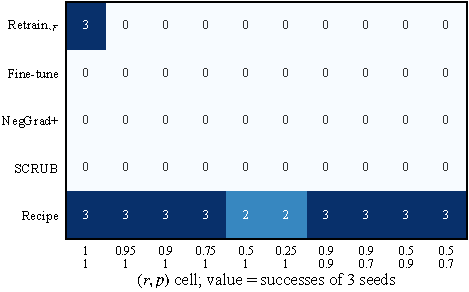
\includegraphics[width=\columnwidth]{fig3_success_map.pdf}
\caption{Number of seeds (of three) meeting both success criteria in each
$(r,p)$ cell. Deletion is dark everywhere except the full-recall corner; the
recipe is dark everywhere except the two lowest-recall cells at $p{=}1$.}
\label{fig:success}
\end{figure}

\subsection{The Grid in Four Views}
Fig.~\ref{fig:views} rearranges the ten cells along four axes. Panel (a) follows
clean accuracy across recall at precision 1.0. Deletion sits on the gold line at
every recall except $r{=}0.95$, where it loses 4.09 points, and $r{=}1$, where it
\emph{is} the gold; SCRUB's damage is concentrated at full recall, where its
three seeds are 57.05\%, 88.83\%, and 51.41\% (mean 65.76\%); the recipe stays
within 1.3 points across the whole range. Panels (b) and (c) are the precision
axes at $r{=}0.9$ and $r{=}0.5$; both are almost flat. Moving $p$ from 1.0 to 0.7
changes deletion's ASR by at most 0.3 points and the recipe's by at most 0.7,
while fine-tuning and SCRUB remain at 100\% and NegGrad+ near its bimodal mean of
33.3\%. Panel (d) isolates the one exception: at $r{=}0.5$, NegGrad+'s clean
accuracy falls from 83.82\% at $p{=}1$ to 57.78\% at $p{=}0.7$. A larger forget
set gives its ascent step more clean samples to damage. That is the only visible
precision effect in the grid, and it belongs to a method that fails at every
precision.

\begin{figure*}[t]
\centering
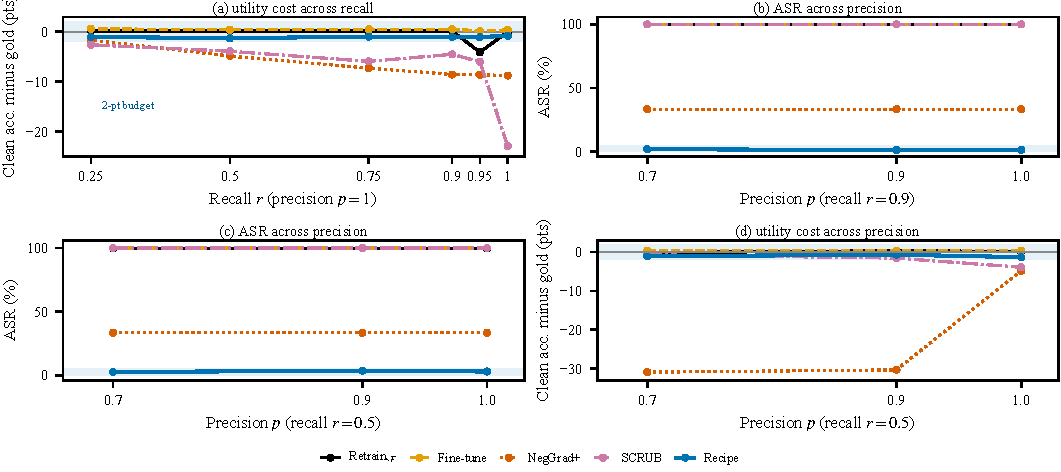
\includegraphics[width=\textwidth]{fig16_grid_views.pdf}
\caption{The E1 grid rearranged. (a) Clean accuracy relative to gold across
recall at $p{=}1$; the shaded band is the two-point budget. (b), (c) ASR across
precision at $r{=}0.9$ and $r{=}0.5$. (d) Clean accuracy relative to gold across
precision at $r{=}0.5$. The recall axis moves every method; the precision axes
move only NegGrad+.}
\label{fig:views}
\end{figure*}

\subsection{Real Detector Columns}
The grid uses simulated forget sets. Table~\ref{tab:e6} checks the conclusion
against the detectors' raw flag sets, with no simulation. Activation clustering
flags exactly the poison at 5\% in this run, and the resulting deletion is a
success (ASR $1.62\%$, clean $88.70\%$). Spectral signatures recovers 83.4\% of
the poison at precision 0.834, and the same deletion method fails completely:
ASR $99.87\%$ with clean accuracy $88.89\%$. The SS column uses the detector's
raw flag set (2{,}500 flags) rather than the fixed $1.5N_p$ budget of
Table~\ref{tab:detector}, so its operating point differs from that table. The
recipe succeeds in both columns
($0.70\%$ and $1.43\%$), and SCRUB fails in both ($100.00\%$). This is the
cleanest statement of the paper's practical claim: a 16.6\% recall shortfall,
which would be an unremarkable detector result, is enough to make the strongest
deletion method useless.

\begin{table}[t]
\centering
\caption{E6: realistic detector columns reproduce the simulated grid.}
\label{tab:e6}
\footnotesize
\begin{tabular}{lcccc}
\toprule
\textbf{Method} & \textbf{Recall} & \textbf{Precision} & \textbf{Clean} & \textbf{ASR} \\
\midrule
Retrain$_{\setminus F}$ & 1.000 & 1.000 & 88.70 & 1.62 \\
SCRUB & 1.000 & 1.000 & 61.37 & 100.00 \\
Recipe & 1.000 & 1.000 & 88.04 & 0.70 \\
Retrain$_{\setminus F}$ & 0.834 & 0.834 & 88.89 & 99.87 \\
SCRUB & 0.834 & 0.834 & 86.89 & 100.00 \\
Recipe & 0.834 & 0.834 & 88.18 & 1.43 \\
\bottomrule
\end{tabular}
\par\vspace{1pt}\footnotesize\raggedright Removal driven by the detectors' \emph{raw} flag sets (no simulation), seed 0. AC flags exactly the poison here; SS trades 16.6\% of recall for 16.6\% precision. Deletion inherits the detector's recall error directly; repair$+$inoculation does not.
\end{table}


\section{Beyond One Setting: Architecture, Attack, and Trigger Knowledge}
\label{sec:general}

\subsection{The Cliff Transfers}
Table~\ref{tab:e7} repeats the critical cells on three settings: VGG-16-BN with
BadNets, VGG-16-BN with Blend, and ResNet-18 with Blend. ResNet-18/BadNets is
already covered by the grid. In every setting, deletion at recall 0.75 or 0.5
fails completely: ASR is 99.42--100.00\% and clean accuracy is indistinguishable
from gold. In every setting, the recipe at the same recall holds ASR at or below
$1.02\%$. The largest clean-accuracy cost is 4.09 points, in the VGG-16-BN/Blend
cell at $r{=}0.5$ ($84.80\%$ against a gold of $88.89\%$); VGG-16-BN/BadNets
costs 3.26 points at the same recall. ResNet-18 is cheaper: 2.60 points for
Blend at $r{=}0.75$ and 2.04 points at $r{=}0.5$. The recipe is thus not free, and its cost grows with the
depth of the architecture and the strength of the trigger, but it remains inside
a plausible budget where deletion is not.

Fig.~\ref{fig:e7} shows the same cells on a log scale. Panel (a) separates the
two outcomes: every deletion cell is at 99.42--100.00\%, more than an order of
magnitude above the 5\% line, while every recipe cell is at 0.29--1.02\%. Panel
(b) is the price. Deletion is within 0.7 points of gold in every cell, because
the poison it fails to remove also does not change clean accuracy at this scale.
The recipe's cost is ordered by trigger strength first and depth second: 1.71 and
3.26 points for VGG-16-BN/BadNets at $r{=}0.75$ and $0.5$; 2.99 and 4.09 for
VGG-16-BN/Blend; 2.60 and 2.04 for ResNet-18/Blend. The cost exceeds three points
at $r{=}0.5$ on VGG-16-BN for both attacks (3.26 points with BadNets and 4.09
with Blend).

\begin{figure}[t]
\centering
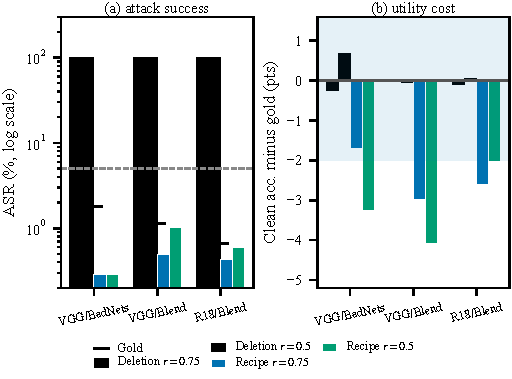
\includegraphics[width=\columnwidth]{fig17_e7_transfer.pdf}
\caption{The transfer settings. (a) ASR after deletion and after the recipe at
recall 0.75 and 0.5, on a log scale; the dashed line is 5\%. (b) Clean accuracy
relative to each setting's gold model; the shaded band is the two-point budget.
Deletion stays within 0.7 points of gold and does not remove the backdoor; the
recipe removes it at a cost of 1.7--4.1 points.}
\label{fig:e7}
\end{figure}

The transfer matters because the cliff could have been an artefact of one
architecture's optimisation. It is not. The step appears in a network with batch
normalisation at every layer and in one with a different depth and width, under a
local patch trigger and under a global blend trigger. The location of the step
does not move: it lies between full removal and partial removal at 75\%,
consistent with the E1 boundary between 95\% and 90\% recall.

\begin{table}[t]
\centering
\caption{E7: the cliff and the recipe's tolerance transfer across architecture and attack.}
\label{tab:e7}
\footnotesize
\setlength{\tabcolsep}{4pt}
\begin{tabular}{lccc}
\toprule
\textbf{Method} & \shortstack{\textbf{VGG-16-BN}\\\textbf{BadNets}} & \shortstack{\textbf{VGG-16-BN}\\\textbf{Blend}} & \shortstack{\textbf{ResNet-18}\\\textbf{Blend}} \\
\midrule
Gold & 88.95 / 1.80 & 88.89 / 1.14 & 88.75 / 0.66 \\
Deletion, $r{=}0.75$ & 88.71 / 100.00 & 88.93 / 99.42 & 88.64 / 99.70 \\
Deletion, $r{=}0.5$ & 89.64 / 100.00 & 88.83 / 99.84 & 88.81 / 99.94 \\
Recipe, $r{=}0.75$ & 87.24 / 0.29 & 85.90 / 0.49 & 86.15 / 0.43 \\
Recipe, $r{=}0.5$ & 85.69 / 0.29 & 84.80 / 1.02 & 86.71 / 0.60 \\
\bottomrule
\end{tabular}
\par\vspace{1pt}\footnotesize\raggedright Cells are clean accuracy / ASR (\%). Gold is the oracle retrain at $r{=}1$. Deletion fails at both recall levels for every architecture--attack pair; the recipe holds ASR $\leq1.02\%$, at a clean-accuracy cost of up to 4.09 points at $r{=}0.5$.
\end{table}


\subsection{The Recipe's Tolerance Is Bought With Trigger Knowledge}
The recipe's advantage comes from its inoculation stage, which presents the
trigger to the network with the correct label. That step requires the trigger. In
the grid, and in Table~\ref{tab:e7}, the true trigger is used. This is a
known-trigger upper bound, and it is essential to say so: a defence that must be
told the trigger is not a blind defence, and a practitioner who does not know the
trigger cannot run the recipe in the form that produces these numbers.

To measure how much the bound is worth, we replace the true trigger with one
synthesised from the poisoned model by the Neural Cleanse procedure described in
Section~\ref{sec:methods}. Table~\ref{tab:e7b} reports the result. On
ResNet-18/BadNets the synthesised mask has zero intersection with the true
$4\times4$ patch (IoU $=0.000$), and inoculation with it leaves ASR at
$98.99\%$ with clean accuracy $87.67\%$. On ResNet-18/Blend the synthesised mask
has a soft mass of about 166 pixels, roughly ten times the 16 pixels of the true
patch, and inoculation with it leaves ASR at $95.72\%$ with clean accuracy
$87.32\%$. In other words, the synthesis stage recovers a mask that is large and
diffuse, not the compact patch that the attack uses, and the inoculation built on
it does not remove the backdoor.

This is the strongest negative result in the paper, because it closes the obvious
escape route. One might hope that a defence could use the recipe's tolerance
without knowing the trigger, by synthesising the trigger first. On these two
attacks, that composition fails at the first step. The recipe is therefore best
read as a ceiling: it shows what trigger-aware repair can achieve under imperfect
recall, and it bounds from above what any trigger-synthesis-based defence could
achieve if synthesis were perfect. It does not demonstrate a deployable method.

\begin{table}[t]
\centering
\caption{E7b: replacing the true trigger with a synthesised one destroys the
recipe's advantage.}
\label{tab:e7b}
\footnotesize
\begin{tabular}{lcccc}
\toprule
\textbf{Setting} & \textbf{Clean} & \textbf{ASR} & \textbf{IoU} & \textbf{Mask mass} \\
\midrule
R18/BadNets & 87.67 & 98.99 & 0.000 & -- \\
R18/Blend & 87.32 & 95.72 & -- & 166 \\
\bottomrule
\end{tabular}
\par\vspace{1pt}\footnotesize\raggedright Inoculation with a synthesised trigger,
recall 1.0. The true BadNets patch occupies 16 pixels; the synthesised Blend mask
has a soft mass of 166 pixels, about ten times larger. With the true trigger the
recipe holds ASR at $0.63\%$ on ResNet-18/BadNets at $r{=}1$
(Table~\ref{tab:e1grid}) and at $0.43$--$0.60\%$ on ResNet-18/Blend at
$r{=}0.75$ and $0.5$ (Table~\ref{tab:e7}). IoU and mask mass were not both logged
for every cell; the table reports what each run recorded.
\end{table}

\subsection{Which Component Does the Work?}
The E1 grid contains an inoculation-only baseline ($17.67\%$ ASR) and the E8
block contains a label-repair-only baseline ($8.63$--$16.36\%$ ASR, discussed in
Section~\ref{sec:calib}). Neither alone crosses the 5\% threshold; the
combination does, at $0.63$--$2.95\%$ across the grid. The two stages are
complementary rather than redundant. Repair removes the label noise that would
otherwise teach the network to associate the trigger with the target; inoculation
changes the association even for poison that never entered the forget set. The
first is bounded by recall, the second is bounded by trigger knowledge. The
recipe works in the middle ground where each covers the other's weakness.

This decomposition also explains why the recipe degrades gracefully rather than
catastrophically. At $r{=}0.5$, half the poison is still in the training set,
but its labels have been repaired (for the half that was flagged) and the trigger
has been re-labelled for the whole network through inoculation. The residual
association is weak, and ASR sits at 2--4\% rather than at 100\%. At $r{=}0.25$
the repair covers too little of the poison for the inoculation to dominate, and
ASR rises to 5.42\%. The transition is gradual because it reflects a balance
between two mechanisms, not a threshold in the data.

\subsection{Poison Rate}
The amplification study (Section~\ref{sec:calib}) runs at a 10\% poison rate and
therefore provides a second scale. At that rate, a partial label repair without
inoculation lowers ASR from 99.99\% to between 11.07\% and 33.03\% depending on
seed and strength. That is a substantial reduction, but it is not a removal by
our criterion, and it occurs in a regime where the detector itself is weakest:
activation clustering returns no flags at 10\%, and spectral signatures recovers
48.0\% of the poison. The combination of a harder attack and a worse detector is
exactly the regime in which a controlled study is most useful, because it is
where the difference between a method that needs recall and a method that does
not becomes visible. We do not claim that the recipe's tolerance is
rate-independent; the 10\% block does not include the full recipe, and we did not
run the full grid at 10\%.

\section{Calibration and Amplification Fail}
\label{sec:calib}

The grid says that trigger-aware repair is the only family that tolerates
imperfect recall, and that it needs the trigger. Two natural responses are to
avoid the trigger requirement through calibration and to rescue deletion by
making the poison it missed easier to find. We tried both. Neither works under
our pre-registered criteria.

\subsection{Calibrate-then-Remove}
CaR uses a synthesised trigger as a proxy for the real one. For each
spectral-signature threshold $\theta$, it builds the corresponding forget set,
runs the recipe's repair stage, and measures the proxy-removed model's response
$\tau$ to the synthesised pattern. A threshold is acceptable only if
$\tau\leq5\%$, because a model that no longer responds to the proxy is presumed
not to respond to the real trigger either. If no threshold qualifies, the method
falls back to the F1-optimal one.

Table~\ref{tab:car} reports the sweep. Across twenty thresholds, $\tau$ is
100\% in nineteen cases and 97.5\% in the remaining one. The proxy pattern is
optimised on the poisoned model and has zero intersection with the true patch, so
label repair does not remove the model's response to it; the calibration signal
is saturated regardless of how much poison the threshold captures. The recall of
the sweep ranges from 0.003 to 1.000 and its precision from 0.333 to 1.000, so
the sweep does cover the useful range. The best F1 is 0.918 at recall 0.894 and
precision 0.942, and the model produced there still has ASR $99.97\%$ and clean
accuracy $86.71\%$. The CaR rule never fires, the fallback is taken, and the
fallback does not remove the backdoor.

The failure is instructive. A calibration guarantee is only as good as the
exchangeability between the calibration signal and the test signal. Here the
proxy is a different pattern, optimised for a different purpose, and the repair
stage is not designed to suppress it. The guarantee is vacuous before any
threshold is chosen.

\begin{table}[t]
\centering
\caption{E3: Calibrate-then-Remove fails because the proxy signal is uninformative.}
\label{tab:car}
\footnotesize
\begin{tabular}{ccccccc}
\toprule
\textbf{$\theta$} & \textbf{Recall} & \textbf{Precision} & \textbf{$\tau$} & \textbf{F1} & \textbf{Clean} & \textbf{ASR} \\
\midrule
0.01 & 1.000 & 0.333 & 97.5 & 0.500 & 82.32 & 99.78 \\
20.71 & 1.000 & 0.396 & 100.0 & 0.567 & 88.01 & 100.00 \\
35.33 & 0.998 & 0.486 & 100.0 & 0.654 & 88.77 & 100.00 \\
50.23 & 0.992 & 0.628 & 100.0 & 0.769 & 88.88 & 100.00 \\
74.23 & 0.956 & 0.863 & 100.0 & 0.907 & 89.19 & 100.00 \\
127.71 & 0.633 & 0.999 & 100.0 & 0.775 & 89.20 & 100.00 \\
191.72 & 0.161 & 1.000 & 100.0 & 0.277 & 89.29 & 99.98 \\
291.83 & 0.003 & 1.000 & 100.0 & 0.006 & 89.22 & 99.98 \\
\midrule
F1-optimal & 0.894 & 0.942 & 100.0 & 0.918 & 86.71 & 99.97 \\
\bottomrule
\end{tabular}
\par\vspace{1pt}\footnotesize\raggedright Calibrate-then-Remove, seed 0. $\theta$ is the Spectral-Signature threshold, $\tau$ the trigger response of the proxy-removed model (\%). Nineteen of twenty thresholds give $\tau{=}100\%$ and the twentieth $97.5\%$: the synthesised trigger never elicits the backdoor (IoU $=0.000$ against the true patch), so no threshold satisfies $\tau\leq5\%$ and CaR degenerates to its fallback. Both the F1-optimal and the CaR choice leave ASR $\approx100\%$.
\end{table}


\subsection{The Ascent Artefact}
A second attempted rescue is to forget harder. Feature-space ascent on the forget
set is a standard unlearning baseline, and in our first runs it appeared to work:
at learning rate $10^{-3}$ for two epochs, ASR fell to $0.18\%$ and at four
epochs to $0.00\%$ (Table~\ref{tab:e8}, Fig.~\ref{fig:ascent}). Clean accuracy
fell with it, to $85.29\%$ and then to $77.25\%$, which we initially read as the
usual utility cost of unlearning.

The reading was wrong. Batch normalisation maintains running estimates of
activation statistics, and ascent updates them along with the weights. Re-running
the identical schedules with the batch-norm statistics frozen to those estimated
on the retained set removes the apparent effect entirely: ASR is
$99.94$--$99.98\%$ at every learning rate, with clean accuracy $88.72$--$88.74\%$
and no utility loss at all. The backdoor was never removed; the normalisation
layers were corrupted, and the corrupted statistics made the trigger inoperative
while also damaging clean accuracy. A reader who evaluates unlearning without a
normalisation control can therefore report a successful removal that is an
artefact of the evaluation pipeline.

Label repair at comparable strength behaves differently. At learning rate
$0.005$ for two epochs ASR is $10.11\%$ with clean accuracy $87.91\%$; at $0.01$
for one epoch it is $16.36\%$ with $87.15\%$; a re-run of the same cells gave
$8.63\%$ and $15.11\%$. These are genuine reductions, achieved without damaging
the network, but they are above the 5\% threshold. Repair needs the inoculation
stage to cross it.

\begin{table}[t]
\centering
\caption{E8: ascent-based 'removal' is a normalisation artefact.}
\label{tab:e8}
\footnotesize
\begin{tabular}{llcc}
\toprule
\textbf{Variant} & \textbf{Setting} & \textbf{Clean} & \textbf{ASR} \\
\midrule
Raw ascent & lr0.0002 ep2 & 88.03 & 18.06 \\
Raw ascent & lr0.0005 ep2 & 87.31 & 2.87 \\
Raw ascent & lr0.001 ep2 & 85.29 & 0.18 \\
Raw ascent & lr0.001 ep4 & 77.25 & 0.00 \\
BN-guarded ascent & lr0.0002 ep2 & 88.74 & 99.98 \\
BN-guarded ascent & lr0.0005 ep2 & 88.72 & 99.98 \\
BN-guarded ascent & lr0.001 ep2 & 88.72 & 99.97 \\
BN-guarded ascent & lr0.001 ep4 & 88.73 & 99.94 \\
Label repair & lr0.005 ep2 & 87.91 & 10.11 \\
Label repair & lr0.01 ep1 & 87.15 & 16.36 \\
Label repair (v2) & lr0.005 ep2 & 87.94 & 8.63 \\
Label repair (v2) & lr0.01 ep1 & 87.45 & 15.11 \\
\bottomrule
\end{tabular}
\par\vspace{1pt}\footnotesize\raggedright Seed 1. Raw feature-space ascent appears to remove the backdoor only by destroying the network: clean accuracy falls from $88.03\%$ at the gentlest setting to $77.25\%$ at lr $10^{-3}$ for four epochs, 11.4 points below the gold mean. Re-running the identical schedule with batch-norm statistics frozen to the retain set leaves ASR at $\approx100\%$: the apparent removal was BN corruption, not unlearning. Label repair at the same strength reduces ASR while keeping clean accuracy within 1.5 points.
\end{table}


\begin{figure}[t]
\centering
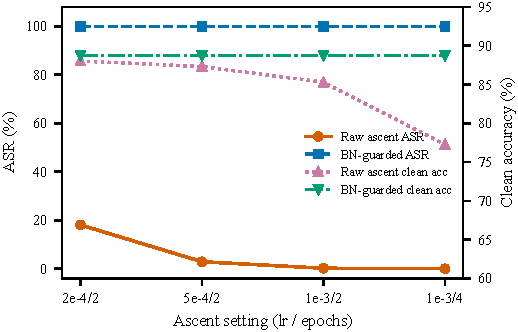
\includegraphics[width=\columnwidth]{fig5_e8_ascent.pdf}
\caption{Raw feature-space ascent appears to remove the backdoor while clean
accuracy collapses; the identical schedules with batch-norm statistics frozen to
the retain set leave ASR at 100\%. The apparent removal is a normalisation
artefact.}
\label{fig:ascent}
\end{figure}

\subsection{The Amplification Hypothesis}
If partial unlearning cannot remove the missed poison, can it at least make that
poison easier to detect afterwards? The hypothesis is plausible: if the network
must support the backdoor on a smaller set of poisoned samples, it may allocate
more capacity to them, and their representations may separate more cleanly from
clean data. If true, the right response to imperfect recall would be an
amplify-and-detect loop: partially remove, re-detect the residue, remove again.

We tested the hypothesis with a pre-registered promotion gate. Partial label
repair was applied at two strengths on the 5\%-poison ResNet-18/BadNets and
ResNet-18/Blend models, and a spectral-signature score was fitted to separate
the missed poison from clean target-class data. The gate required an AUC gain of
at least $+0.10$ over the base model, a clean-accuracy loss of at most two
points, and a gain larger than a matched control that received the same
intervention on clean data instead of poison, on all seeds.

Fig.~\ref{fig:spike} shows the outcome on two seeds. The base models sit at AUC
0.507--0.549 with ASR 99.6--99.8\% and clean accuracy 63.5--63.9\%. Six repaired
models were run. All of them reduce ASR (to between 0.31\% and 87.85\%) and all
raise AUC relative to their base, to between 0.569 and 0.672. But every one of
them also loses clean accuracy: the smallest loss is 2.2 points, and the range is
53.9--61.3\%. The highest AUC, 0.672, occurs at ASR $0.31\%$ and clean accuracy
$55.68\%$; the next, 0.650, at ASR $58.44\%$ and clean accuracy $59.58\%$. The matched
clean-removal controls, which apply the same procedure to clean data instead of
poison, stay at AUC 0.494--0.550 with clean accuracy 62.3--63.3\%. The pattern is
that of a damaged network whose features separate everything a little better, not
of a backdoor made salient: the amplification signal and the utility loss arrive
together. No repaired row remains within two points of its base clean accuracy,
so the pre-registered gate fails on the utility clause even in the rows where the
AUC clause passes.

\begin{figure}[t]
\centering
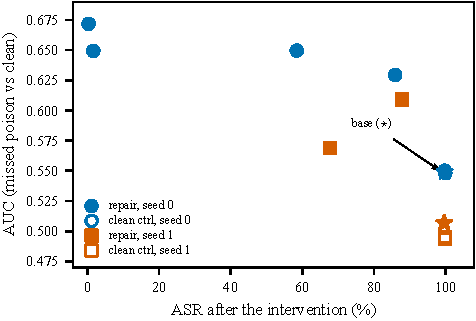
\includegraphics[width=\columnwidth]{fig11_spike_auc.pdf}
\caption{Detectability of missed poison after partial label repair. Filled
markers are repaired models, open markers are matched clean-removal controls,
stars are the poisoned base. AUC rises only where clean accuracy has fallen by
2--10 points; the controls stay at chance.}
\label{fig:spike}
\end{figure}

\subsection{Full-Scale Test}
The spike used 5\% poison and a partial repair. To test the hypothesis at the
scale where it would matter, we repeated it with 10\% poison, three seeds, two
repair strengths, and matched controls (Table~\ref{tab:e9}, Fig.~\ref{fig:amplify}).
The base models have AUC 0.494--0.499. Repair at learning rate $0.005$ gives
0.470--0.497; repair at $0.01$ gives 0.468--0.500. The controls give
0.492--0.503. Every value is at chance, and the largest gain over the base mean
of 0.496 is 0.006. It comes from a control, not from a repaired model; the
largest repair gain is 0.003. Both are two orders of magnitude below the gate of
$+0.10$.

The repair does reduce ASR, from 99.99--100.00\% to 11.07--33.03\%, and it does
so with clean accuracy between 86.81 and 88.20\%, within the two-point budget of
the gold models on every seed. So partial repair is a real
mitigation. What it is not is an amplifier: the poison it fails to remove is no
easier to detect than before. The pre-registered gate fails on its AUC clause on
every seed; it also fails the control clause, because the controls are at chance
and therefore not distinguishable from the repair in the direction the hypothesis
predicts.

\begin{table}[t]
\centering
\caption{E9: the amplification effect does not survive at full scale.}
\label{tab:e9}
\footnotesize
\setlength{\tabcolsep}{5pt}
\begin{tabular}{lccc}
\toprule
\multicolumn{4}{@{}l}{\emph{(a) AUC separating missed poison from clean class-0 data}}\\
\textbf{Condition} & \textbf{Seed 0} & \textbf{Seed 1} & \textbf{Seed 2} \\
\midrule
Base & 0.494 & 0.499 & 0.496 \\
Repair, lr 0.005 & 0.470 & 0.497 & 0.487 \\
Repair, lr 0.01 & 0.468 & 0.476 & 0.499 \\
Clean control, lr 0.005 & 0.492 & 0.499 & 0.501 \\
Clean control, lr 0.01 & 0.495 & 0.503 & 0.501 \\
\midrule
\multicolumn{4}{@{}l}{\emph{(b) Repair outcomes (lr 0.005 / lr 0.01)}}\\
\textbf{Seed} & \textbf{ASR (\%)} & \textbf{Clean acc.\ (\%)} & \\
\midrule
0 & 11.1 / 33.0 & 88.2 / 86.8 & \\
1 & 15.9 / 17.7 & 88.1 / 86.9 & \\
2 & 21.3 / 29.6 & 88.1 / 87.3 & \\
\bottomrule
\end{tabular}
\par\vspace{1pt}\footnotesize\raggedright 10\% poison, simulated recall-0.5 flags. AUC separates the 2{,}500 \emph{missed} poison samples from clean class-0 data. Partial label repair lowers ASR but does not raise AUC above the base model by more than $0.003$ in any seed; the matched clean-removal controls keep ASR at 99.94--100.00\% and clean accuracy at 86.7--87.8\%, and their AUC sits at chance. The pre-registered promotion gate ($\geq+0.10$ AUC, $\leq2$ points clean loss, beating control) fails on every clause.
\end{table}


\begin{figure}[t]
\centering
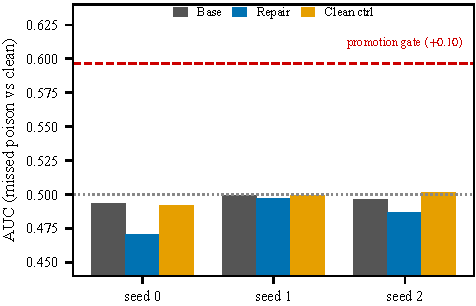
\includegraphics[width=\columnwidth]{fig6_e9_amplify.pdf}
\caption{AUC separating missed poison from clean target-class data at 10\%
poison, three seeds. Partial repair (red) and matched clean-removal controls
(orange) both sit at chance; the dashed line is the pre-registered promotion
gate at base $+0.10$.}
\label{fig:amplify}
\end{figure}

\subsection{What the Failures Have in Common}
Both refinements try to avoid the recipe's dependence on the trigger, and both
fail for the same underlying reason: they need a signal that distinguishes poison
from clean data without knowing what the trigger is. CaR's proxy is a different
pattern and is never suppressed; the amplification hypothesis assumes that the
residual poison becomes more salient, and it does not. The only method in our
suite that crosses the 5\% threshold under imperfect recall is the one that uses
the true trigger. That is a negative result about the state of post-training
removal, and we report it as one.

\section{Durability and Efficiency-Oriented Baselines}
\label{sec:durability}

\subsection{Relearning the Removed Backdoor}
A removal that leaves the model unable to express the backdoor today may still
leave it able to relearn it tomorrow. We test this on the gold model, the
oracle-deleted network that every removal method is trying to approximate. The
probe gives the model one hundred freshly poisoned samples, trains for a small
number of steps, and measures ASR. The samples are generated with the same
trigger and target as the original attack but were not in the original training
set.

Table~\ref{tab:durability} and Fig.~\ref{fig:relearn} report the result. At step
zero the gold model's ASR is 0.6--1.2\%. After five steps it is 4.7\% for
VGG-16-BN/BadNets, 25.2\% for ResNet-18/BadNets, 78.2\% for VGG-16-BN/Blend, and
96.0\% for ResNet-18/Blend. After ten steps every setting is at or above 97.6\%,
and it stays there through fifty steps. One hundred samples are 0.2\% of the
training set. The removed backdoor is not gone; it is dormant, and it returns as
soon as the association is shown again.

The representational fingerprint tells the same story from the other side. A
loss-threshold membership-inference attack on the gold model has AUC
0.491--0.496, indistinguishable from chance, which is what we would expect if the
poisoned samples had been properly removed. The probe is deliberately simple;
stronger membership-inference attacks exist \cite{carlini_mia}, so the
chance-level result should be read as the absence of an easy membership signal
rather than as proof that none exists. The Kullback--Leibler divergence
between the model's outputs on clean and trigger-stamped inputs is zero in both
cases, whereas the poisoned model shows 0.110--0.157 on clean inputs and
12.0--28.2 on trigger-stamped inputs. By both standard tests the removal looks
complete. The relearning probe shows that it is not.

This is the vision-domain analogue of the language-model result of Hu \etal{}
\cite{jogging}, and it has a practical consequence for evaluation: a removal
claim that does not include a relearning probe is a claim about the model's
current behaviour, not about the data it was trained on. We did not run the
relearning probe on the recipe's output, because the recipe keeps and relabels
the flagged data rather than deleting it; whether its dormancy is longer or
shorter than the gold model's is an open question that our records cannot answer.

\begin{table}[t]
\centering
\caption{E5: durability probes on the oracle-deleted model.}
\label{tab:durability}
\footnotesize
\setlength{\tabcolsep}{5pt}
\begin{tabular}{lcccc}
\toprule
\multicolumn{5}{@{}l}{\emph{(a) Relearning: ASR (\%) after $k$ steps on 100 fresh poison samples}}\\
\textbf{Setting} & \textbf{Step 0} & \textbf{Step 5} & \textbf{Step 10} & \textbf{Step 50} \\
\midrule
R18/BadNets & 1.2 & 25.2 & 100.0 & 99.9 \\
R18/Blend & 0.6 & 96.0 & 99.3 & 98.7 \\
VGG/BadNets & 1.2 & 4.7 & 97.7 & 99.9 \\
VGG/Blend & 0.6 & 78.2 & 99.9 & 98.9 \\
\midrule
\multicolumn{5}{@{}l}{\emph{(b) Representational probes on the same model}}\\
\textbf{Setting} & \textbf{MIA AUC} & \textbf{KL clean} & \textbf{KL trigger} & \\
\midrule
R18/BadNets & 0.495 & 0.000 & 0.0 & \\
R18/Blend & 0.495 & 0.000 & 0.0 & \\
VGG/BadNets & 0.491 & 0.000 & 0.0 & \\
VGG/Blend & 0.493 & 0.000 & 0.0 & \\
\bottomrule
\end{tabular}
\par\vspace{1pt}\footnotesize\raggedright The gold (oracle-deleted) model, i.e.\ the best case any removal method can reach. One hundred fresh poisoned samples restore ASR to $\geq97.6\%$ within 10 steps in all four settings; the loss-threshold MIA sits at chance (0.49--0.50); and the clean-vs-trigger KL gap that characterises a live backdoor (0.11--0.16 vs.\ 12--28 in the poisoned model) has vanished. Suppression, not erasure.
\end{table}


\begin{figure}[t]
\centering
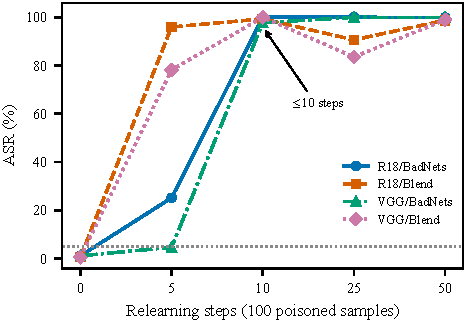
\includegraphics[width=\columnwidth]{fig9_relearn.pdf}
\caption{ASR of the oracle-deleted gold model after $k$ gradient steps on one
hundred fresh poisoned samples. All four settings return to at least 97.6\% ASR
within ten steps.}
\label{fig:relearn}
\end{figure}

\subsection{What the Probes Can and Cannot Certify}
Fig.~\ref{fig:probes} places both probes on the same axis, the fraction of poison
removed. Panel (a) is the membership-inference AUC. It is at chance at every
fraction, including the fully poisoned model, so on these models it cannot
certify anything about poison: the probe never had a signal to lose. This matters
because an AUC near 0.5 is sometimes reported as evidence of successful
unlearning. Here it is evidence only that the training procedure leaves no
detectable membership trace, which was already true before removal. Panel (b) is
the KL divergence between the model's outputs on clean and trigger-stamped
inputs. It stays between 12.0 and 28.2 while any poison remains and falls to zero
only when every poisoned sample is removed. Unlike the membership probe, it
tracks the poison, but it certifies current behaviour rather than the absence of
the capability: at 100\% removal it reads zero on the same gold model that
relearns to 97.7\% ASR within ten steps.

\subsection{SISA}
SISA-5 is the strongest efficiency-oriented alternative in our suite: it removes
the backdoor at full recall, reaching ASR $3.04\%$ with clean accuracy
$70.38\%$. The clean accuracy is 18.3 points below the frozen gold model, so the
run fails the joint criterion by a wide margin. At recall 0.5 the ASR is
$100.00\%$ and the clean accuracy $67.49\%$: the method inherits the same recall
cliff as deletion, on top of its sharding cost. The pilot runs with ten and
twenty shards are worse still ($50.25\%$ clean at ASR $6.26\%$, and $37.59\%$ at
$8.04\%$), which is the expected direction: more shards mean less data per
constituent model and a larger utility penalty. SISA's guarantee is about the
data that is forgotten, not about the data that is missed, and it does not change
the cliff.

\subsection{Fine-Pruning}
Fine-pruning removes the filters with the smallest average activation on clean
data. On ResNet-18/BadNets, pruning 40\% of channels leaves ASR at $63.64\%$ and
clean accuracy at $65.50\%$; pruning 60\% reaches ASR $0.00\%$ with clean
accuracy $61.30\%$. On VGG-16-BN/BadNets the method needs 90\% of channels before
ASR falls to zero, at which point clean accuracy is $67.85\%$. The base models in
this block are weaker than the frozen gold (69.5\% and 71.0\% clean), because the
block was run under a shorter schedule, so the absolute numbers are not directly
comparable with Table~\ref{tab:e1grid}. The relative cost is: 8.2 points for
ResNet-18 and 3.1 points for VGG-16-BN from their own bases, plus the 18--19-point
gap between those bases and the frozen protocol. Fine-pruning is also
trigger-agnostic in the wrong sense: it can only remove a backdoor that is
visible as dormant neurons, and it has no mechanism for poison that is
distributed across the network.

\begin{figure}[!tb]
\centering
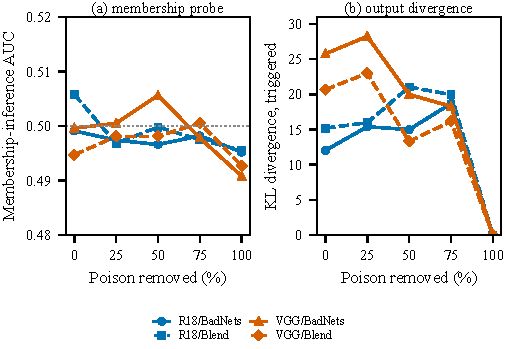
\includegraphics[width=\columnwidth]{fig18_durability_probes.pdf}
\caption{Representational probes on the E2 models as a function of the fraction
of poison removed. (a) Membership-inference AUC is at chance at every fraction,
including the fully poisoned model. (b) KL divergence between clean and
trigger-stamped outputs is high while any poison remains and zero only at full
removal. Neither probe distinguishes suppression from erasure.}
\label{fig:probes}
\end{figure}

\subsection{Pilot Baselines}
Table~\ref{tab:baselines} also lists rows from the earlier pilot protocol. They
are not pooled with the frozen results, and we mark them as pilot rows. Three of
them are informative. Partial deletion of 25\%, 50\%, or 75\% of the poison
leaves ASR between 99.86\% and 100.00\%, which is the same step seen in E2.
Gradient ascent in the pilot leaves ASR at 99.93\% on ResNet-18 and 99.99\% on
VGG-16-BN (mean 99.96\%), consistent with the normalisation artefact diagnosed
in Section~\ref{sec:calib}. Label repair without inoculation averaged ASR
$0.46\%$ at $83.37\%$ clean accuracy over two pilot runs (0.54\%/85.55\% on
ResNet-18 and 0.38\%/81.19\% on VGG-16-BN), a 6.6-point cost against that
protocol's approximately 90\% baseline. It did not reproduce under the frozen
protocol, where label repair alone gave $8.63$--$16.36\%$ ASR with clean accuracy
within 1.5 points. We report both, and we do not use the pilot row to support a
success claim.

\begin{table}[t]
\centering
\caption{Efficiency-oriented and sharded baselines.}
\label{tab:baselines}
\footnotesize
\begin{tabular}{lccc}
\toprule
\textbf{Method} & \textbf{Recall} & \textbf{Clean} & \textbf{ASR} \\
\midrule
SISA-5 (this protocol) & 1.0 & 70.38 & 3.04 \\
SISA-5 (this protocol) & 0.5 & 67.49 & 100.00 \\
SISA-5 (pilot) & oracle & 63.83 & 3.79 \\
SISA-10 (pilot) & oracle & 50.25 & 6.26 \\
SISA-20 (pilot) & oracle & 37.59 & 8.04 \\
Fine-pruning R18, 40\% & -- & 65.50 & 63.64 \\
Fine-pruning R18, 60\% & -- & 61.30 & 0.00 \\
Fine-pruning VGG, 90\% & -- & 67.85 & 0.00 \\
\midrule
Gradient ascent (pilot) & -- & 87.62 & 99.96 \\
Label repair FT (pilot) & -- & 83.37 & 0.46 \\
Partial deletion 25\% (pilot) & -- & 89.97 & 99.98 \\
Partial deletion 50\% (pilot) & -- & 90.13 & 99.96 \\
Partial deletion 75\% (pilot) & -- & 90.08 & 99.96 \\
\bottomrule
\end{tabular}
\par\vspace{1pt}\footnotesize\raggedright Reviewer-facing baselines. SISA and fine-pruning rows are measured; pilot rows use the minor project's earlier protocol (clean accuracy $\approx$90\%) and are shown for completeness, not pooled with the frozen results. Pilot values are means over the runs recorded in the master results table (two architecture variants for SISA and repair, four runs for partial deletion). SISA's clean accuracy is 18 points below the frozen gold model already at $r{=}1$; fine-pruning needs 60\% (ResNet) or 90\% (VGG) of channels pruned before ASR falls, by which point clean accuracy has dropped 8 and 3 points respectively.
\end{table}


\subsection{Summary of the Baselines}
The baselines divide into two groups. Methods that delete data and retrain
(SISA, deletion) can remove the backdoor at full recall, but they pay a utility
cost that ranges from 18 points for SISA-5 to a fraction of a point for deletion,
and they inherit the recall cliff. Methods that edit the model without a
trigger-aware objective (fine-pruning, gradient ascent, retain fine-tuning) either
need to remove most of the network or do not remove the backdoor at all. None of
them reaches the joint criterion at a cost below retraining with full recall. The
recipe is the only method that reaches it at recall 0.5, and it does so with
trigger knowledge that the baselines do not require.

\section{Cross-Domain Replication: Radio Modulation Classification}
\label{sec:rf}

\subsection{Motivation}
The recall cliff could be a property of image classifiers, of convolutional
feature hierarchies, or of the particular detectors we use. To test whether it is
a property of deletion under partial poison, we repeat the core experiment in a
different modality: automatic modulation classification (AMC) on RadioML
2016.10a \cite{radioml,radioml_jstsp}. AMC is a natural second domain for this
question. Models are trained on large captures that may come from crowd-sourced
or third-party receivers, a poisoned capture is cheap to produce, and a backdoor
that maps a specific waveform to a fixed modulation label is a plausible
integrity attack on a receiver. Adversarial and poisoning threats to wireless
classifiers are an active concern in their own right \cite{sadeghi,flowers}, but
backdoor removal under imperfect detection has not, to our knowledge, been
characterised as a function of recall in this domain. The defence pipeline is the
same: detect, form a forget set, remove.

The protocol is summarised in Section~\ref{sec:protocol}. Eleven modulation
classes, SNR from $-20$ to $18$\,dB, $2\times128$ I/Q windows, unit-energy
normalisation, a three-block one-dimensional CNN, 5\% poison to BPSK, and a fixed
burst trigger that sets $I{=}0.9$ and $Q{=}{-}0.9$ on the last eight samples.
Three seeds vary poison placement and initialisation; the 80/20 split is fixed.
The same four methods and the same $(r,p)$ cells are used as in the image study,
including the precision-0.7 probe at $r{=}0.75$.

One feature of this domain changes how the results must be read. RadioML is
evaluated per SNR, and at low SNR the clean classifier is close to chance. We
report per-SNR numbers because they are the domain's native metric, but we mark
the near-chance region explicitly and restrict the interpretation of the recall
tolerance to SNR at or above $-6$\,dB. A defence that reports a low ASR on a
classifier that cannot classify is not a defence.

\subsection{The Attack and the Base Model}
The poisoned base model reaches ASR 99.54\% at 57.66\% clean accuracy, and its
per-SNR ASR is between 98.61\% and 100.00\% at every SNR from $-20$ to $18$\,dB.
That flatness is expected for a trigger that overwrites the end of the window:
the model can learn to read the burst regardless of the noise on the rest of the
signal. Clean accuracy, by contrast, depends strongly on SNR: 8.45\% at
$-20$\,dB, 10.5\% at $-16$, 23.4\% at $-10$, 48.2\% at $-6$, 63.2\% at $-4$,
82.2\% at $0$, and 85--87\% from 4\,dB upward. At $-20$\,dB the classifier is at
chance (9.1\% for eleven classes), so an ASR of 100\% is not evidence that the
backdoor is sophisticated; it is evidence that the trigger is easier to read than
the signal.

\subsection{Deletion Replicates the Cliff}
Table~\ref{tab:rf} and Fig.~\ref{fig:rf} report the removal results. Deletion
works when the forget set is complete: retraining on the retained set with every
poisoned sample removed reaches ASR $2.90\pm1.43\%$ at $r{=}1$ with clean
accuracy $56.83\pm0.57\%$. At $r{=}0.75$ its ASR is $97.16\pm1.84\%$; at $r{=}0.5$
it is $98.41\pm2.18\%$. The step is in the same place as in CIFAR-10: full recall
works, three-quarters recall does not. Fine-tune
never works, at any recall, with ASR $73.87$--$99.66\%$. On the SNR-averaged
cell, the two trigger-aware methods work down to $r{=}0.5$: the recipe reaches
$0.83\pm0.17\%$, $2.35\pm0.43\%$, and $4.02\pm0.86\%$ at the three recall levels,
and inoculation-only reaches $0.28\pm0.05\%$, $1.60\pm0.23\%$, and
$3.83\pm0.23\%$.
At the precision-0.7 cell ($r{=}0.75$), deletion is at 96.9--99.9\% ASR, the
recipe at 1.5--2.2\%, and inoculation-only at 1.4--1.8\%.

Two differences from the CIFAR results deserve comment. First, inoculation-only
succeeds in this domain, whereas on CIFAR-10 it left ASR at 17.67\%. The trigger
here is a simple additive burst on two channels, and the network's response to it
can be overwritten by presenting the burst with the correct label; the CIFAR patch
is spatial and interacts with many channels, and inoculation alone is not enough.
The cross-domain study therefore replicates the deletion cliff and the recipe's
tolerance, but it does not replicate the CIFAR ordering between the two
trigger-aware methods. We report the difference rather than pooling the domains.

Second, the radio task has a much lower clean-accuracy ceiling than CIFAR-10,
which compresses the utility side of the success criterion. A two-point budget
around a 56\% baseline is a tighter relative constraint than a two-point budget
around 89\%, but all methods here stay within about two points of the gold clean
accuracy, so the verdicts are driven by ASR. This is the regime in which the
recall cliff is easiest to see.

\begin{table}[t]
\centering
\caption{Cross-domain replication on RadioML AMC.}
\label{tab:rf}
\footnotesize
\setlength{\tabcolsep}{4.5pt}
\begin{tabular}{lcccc}
\toprule
\textbf{Method} & \textbf{$r{=}1.0$} & \textbf{$r{=}0.75$} & \textbf{$r{=}0.5$} & \textbf{Clean acc} \\
\midrule
Deletion & 2.90$\pm$1.43 & 97.16$\pm$1.84 & 98.41$\pm$2.18 & 56.75$\pm$0.79 \\
Fine-tune & 73.87$\pm$2.33 & 99.48$\pm$0.35 & 99.66$\pm$0.14 & 58.55$\pm$0.38 \\
Recipe & 0.83$\pm$0.17 & 2.35$\pm$0.43 & 4.02$\pm$0.86 & 57.36$\pm$0.50 \\
Inoc. only & 0.28$\pm$0.05 & 1.60$\pm$0.23 & 3.83$\pm$0.23 & 58.40$\pm$0.30 \\
\bottomrule
\end{tabular}
\par\vspace{1pt}\footnotesize\raggedright RadioML 2016.10a, 3 seeds, 5\% poison, synthetic I/Q trigger. Cells are ASR (\%) mean$\pm$s.d.\ over SNR and seeds; the last column is clean accuracy over all runs. The poisoned base reaches ASR 99.54\% at 57.66\% clean accuracy. The $r{=}1.0$ cell of the deletion row is the gold retrain. The recall cliff reproduces: deletion fails at $r\leq0.75$ (per-SNR ASR 90.3--100\% at $r{=}0.75$ and 89.6--100\% at $r{=}0.5$), while trigger-aware repair keeps the SNR-averaged ASR below 5\% to $r{=}0.5$.
\end{table}


\begin{figure*}[t]
\centering
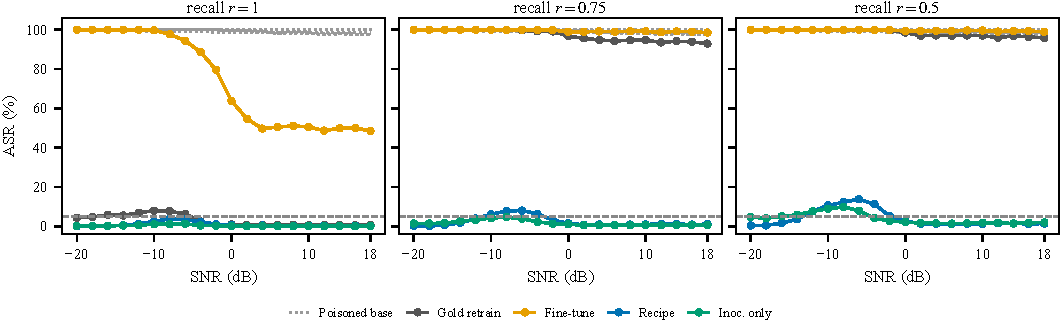
\includegraphics[width=\textwidth]{fig7_rf_asr.pdf}
\caption{ASR versus SNR on RadioML 2016.10a for recall 1.0, 0.75, and 0.5
(mean over three seeds). Deletion succeeds only at full recall (ASR $2.9\%$); at
partial recall its ASR is 90.3--100\%. Fine-tuning never removes the backdoor;
both trigger-aware methods stay at or below 5\% at high SNR, with the recipe
rising at mid SNR as Fig.~\ref{fig:rfheat} shows.}
\label{fig:rf}
\end{figure*}

\subsection{The Tolerance as a Function of SNR}
Fig.~\ref{fig:gamma} plots $\gstar$, the smallest recall at which a method
reaches ASR $\leq5\%$, as a function of SNR. Unlike $\rstar$, $\gstar$ carries no
utility budget: below $-10$\,dB the clean task is itself near chance, so a
two-point accuracy budget would not be meaningful. Clean accuracy is reported
separately in Table~\ref{tab:rf}. The oracle retrain has
$\gstar{=}1.0$ wherever it is defined, and it is undefined between $-16$ and
$-6$\,dB because the oracle model itself sits above 5\% ASR there
(5.45--7.87\%). That undefined region is not a failure of the retrain; it is a
statement that the attack is weak enough at those SNRs that the 5\% threshold
cannot separate a defended model from an undefended one. The two endpoints at
$-20$ and $-18$\,dB, where the oracle reports 4.26\% and 4.63\%, are also
degenerate: gold clean accuracy there is 8.4\% and 10.3\%, at or near chance. We mark
the whole region from $-20$ to $-10$\,dB as near-chance in the figure.

For the trigger-aware methods $\gstar$ is defined in every bin, and the profile
is U-shaped: the requirement is lowest at high SNR, rises through the mid range,
and is uninformative where the clean task is near chance. The recipe has
$\gstar{=}0.75$ at $-12$\,dB, $1.0$ at $-10$ to $-4$\,dB, $0.75$ at $-2$\,dB,
and $0.5$ from $0$\,dB upward. Inoculation-only has a similar profile, between
0.5 and 0.75. Fine-tuning has no $\gstar$: its best cell never falls below
48.5\%. The practical reading is narrower than a single recall number. Above
$0$\,dB, recall 0.5 suffices for trigger-aware repair; at $-12$ and $-2$\,dB the
requirement is 0.75, and between $-10$ and $-4$\,dB it is 1.0; below $-10$\,dB
the clean task is near chance and the criterion is vacuous. Deletion is
insufficient at every SNR at any recall below 1.0. A detector requirement stated
as one number is therefore itself an average over the operating SNR; the
deployment quantity is $\gstar$ as a function of SNR.

\begin{figure}[t]
\centering
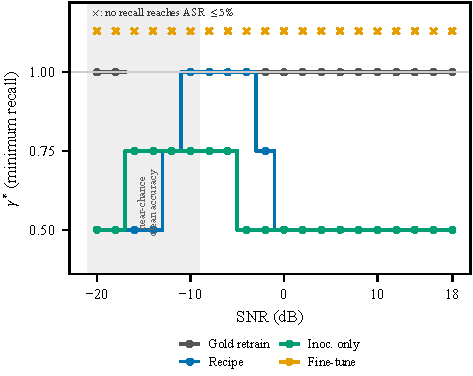
\includegraphics[width=\columnwidth]{fig8_rf_gamma.pdf}
\caption{$\gstar$ (minimum recall reaching ASR $\leq5\%$) versus SNR. Crosses
mark SNRs where no recall qualifies. The shaded region is near-chance clean
accuracy, where the 5\% criterion is vacuous.}
\label{fig:gamma}
\end{figure}

\subsection{Per-SNR Structure}
Fig.~\ref{fig:rfheat} shows every cell as a heatmap. Three structures are
visible. First, the fine-tune row is saturated at the partial-recall columns and
weakens only at $r{=}1$, where it falls from about 100\% in the near-chance bins
to 48.5\% at 18\,dB. That is the CIFAR-10 fine-tuning result at higher
resolution: even its best cell is ten times the 5\% threshold. Second, the
retrain row, which is the oracle at $r{=}1$ and partial deletion below it, turns
from blue to red between the first and second columns at every SNR: it is at
90.3--100\% at $r{=}0.75$ and 89.6--100\% at $r{=}0.5$. Third, the two
trigger-aware rows are blue across the band, but not uniformly. The lighter patch
between $-12$ and $-2$\,dB at $r{=}0.5$ is the mid-SNR hump: the recipe's per-SNR
ASR rises to 13.8\% at $-6$\,dB, even though the SNR-averaged cell mean is
4.02\%.

Fig.~\ref{fig:rfclean} explains why the left edge of the heatmap cannot be read
as a defence. In the shaded region below $-10$\,dB the three curves are
indistinguishable, and at $-20$ and $-16$\,dB they sit within 1.5 points of
chance. Above $-6$\,dB the recipe tracks gold within 4.3 points, so the mid-SNR
hump is a real removal failure on a task the network can perform, not a
side-effect of chance-level features.

\begin{figure*}[t]
\centering
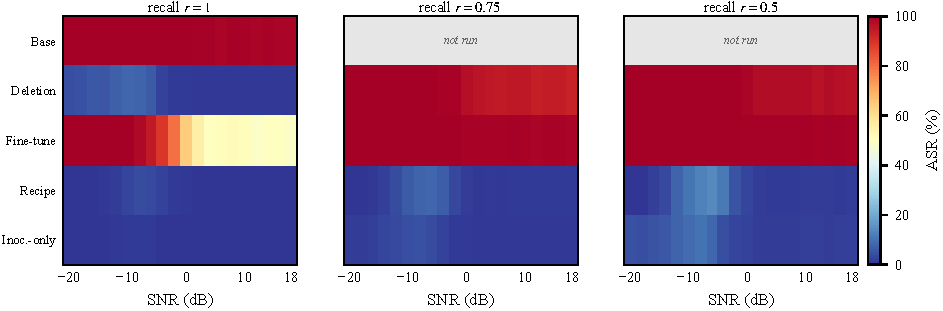
\includegraphics[width=\textwidth]{fig19_rf_heatmap.pdf}
\caption{ASR by SNR and recall for the radio study (mean over three seeds). The
retrain row is the oracle at $r{=}1$ and partial deletion at the lower recalls;
the base row was not run at partial recall (grey). Fine-tuning is saturated
except at full recall above 0\,dB; both trigger-aware methods are blue across the
band, with a lighter patch for the recipe at mid SNR.}
\label{fig:rfheat}
\end{figure*}

\begin{figure}[t]
\centering
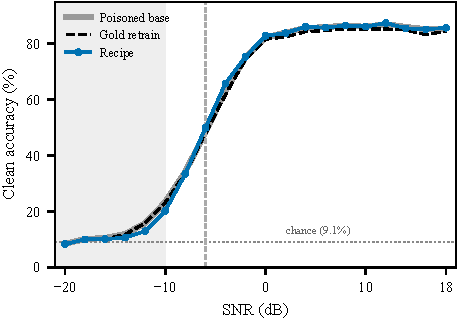
\includegraphics[width=\columnwidth]{fig20_rf_clean.pdf}
\caption{Clean accuracy versus SNR for the poisoned base, the gold retrain, and
the recipe at $r{=}1$. The three curves are nearly indistinguishable; the shaded
region below $-10$\,dB is near chance and the dashed vertical line marks
$-6$\,dB, the lower edge of the interpretable range.}
\label{fig:rfclean}
\end{figure}

\subsection{What the Radio Study Does and Does Not Show}
The study shows that the recall cliff is not specific to images, to
two-dimensional convolutions, or to the two CIFAR detectors. It appears in a
one-dimensional I/Q classifier with a different optimiser, a different poison
mechanism, and a per-SNR evaluation. It also shows that the recipe's tolerance is
not an artefact of the CIFAR architecture, although the simpler trigger makes
inoculation alone sufficient here.

It does not show that the result transfers to over-the-air signals. The trigger
is a digital burst applied before normalisation, not a hardware impairment; the
model is small; the dataset is a standard benchmark with a fixed split; and the
per-SNR bins contain different numbers of samples. These are ordinary
external-validity limits, and we list them rather than claim more than the
experiment supports. Within those limits, the radio study is the strongest
evidence in the paper that the cliff is a property of deletion under partial
poison rather than a property of one benchmark.

\section{Discussion}
\label{sec:discussion}

\subsection{The Cliff Is About Residual Poison}
The grid and the partial-deletion block agree on a simple statement: what
matters is whether any poison remains, not how much was removed. A model trained
on 2{,}250 of 2{,}500 poison samples behaves like a fully poisoned model; a model
trained on 125 behaves like a nearly clean one. The transition is sharp enough
that the difference between a detector with 90\% recall and one with 100\% recall
is the difference between no defence and a complete defence. This is why the
success tolerance of deletion is exactly $\rstar{=}1.00$ rather than a value
slightly below one.

The result is an empirical statement about this family of attacks and models, not
a theorem. A trigger with a smaller effective support, a lower poison rate, or a
model with more capacity might move the step. But the step was in the same place
across two architectures, two triggers, and two modalities, and it was visible
from both directions (increasing recall in the grid, increasing residual poison
in E2). We would be surprised if it moved far under moderate changes to the
protocol.

\subsection{Detector Engineering Should Optimise Recall}
The precision axis is nearly flat. At fixed recall, adding clean false positives
to the forget set changes ASR by less than a point for deletion and by a small,
non-monotone amount for the recipe. The cost appears on the utility side, where
the recipe loses at most about 0.6 points across the precision cells. This
suggests a division of labour: detector design should maximise recall subject to
a precision floor that keeps the forget set affordable, and removal design should
assume that the forget set will contain clean data.

The activation-clustering result at 10\% poison is a warning about detector
design as much as about removal. The detector returns nothing at exactly the
poison rate where the attack is strongest, because its cluster-size threshold
assumes that poison is a small minority. A detector that cannot flag a large
poison fraction is not conservative; it is silently permissive. Reporting recall
and precision at a single poison rate would not have revealed this.

\subsection{Why Trigger-Aware Repair Tolerates Half the Poison}
The recipe does not need to identify every poisoned sample because its
inoculation stage changes the trigger-to-target association for the whole
network. Label repair removes the label noise that would otherwise re-teach the
association on the flagged subset; inoculation teaches the network that the
trigger is uninformative on a large sample of clean data. The two mechanisms
cover different failures: repair handles the poison that was found, inoculation
handles the poison that was missed, up to a point. The balance breaks at
$r{=}0.25$, where three-quarters of the poison keeps its original label and the
inoculation signal is not enough.

This also explains why the recipe's clean-accuracy cost grows with architecture
depth and trigger strength. Inoculation is a data-dependent regulariser, and the
network must fit both the retained data and the re-labelled trigger examples. The
cost is small (about one point) on ResNet-18 and larger (up to 4.1 points) on
VGG-16-BN with Blend, which is the setting with the largest distribution shift
between clean and trigger-stamped inputs.

\subsection{The Known-Trigger Bound Is the Central Limitation}
The recipe's tolerance is bought with the true trigger, and the synthesis
experiment shows that the purchase cannot be avoided by estimating the trigger
from the model. On both CIFAR attacks the synthesised mask had zero or near-zero
overlap with the true patch, and inoculation with it left ASR above 95\%. This
places the recipe on the ceiling side of the problem: it is a strong upper bound
on what post-training repair can do, and it is not a blind defence.

The bound matters for how the paper should be cited. A reader should not take
away ``repair removes backdoors at 50\% recall''. The correct takeaway is
``repair removes backdoors at 50\% recall if the trigger is known; if it is not,
no method in this study does''. The first statement is a benchmark result. The
second is the deployment result.

\subsection{Relation to Prior Work}
Our findings are consistent with the negative result of Pawelczyk \etal{} for
approximate unlearning \cite{pawelczyk}, and they add a controlled curve that
separates the effect of missed poison from the effect of deleted clean data. They
are also consistent with the relearning result of Hu \etal{} \cite{jogging}: the
oracle-deleted model looks clean by membership inference and by output
divergence, yet relearns the backdoor in ten steps. The difference is that our
probe is a vision classifier and the poison is a trigger, not a text corpus, so
the dormancy is not a language-model artefact.

The ascent artefact is, as far as we know, under-reported. Evaluations of
unlearning that use feature-space ascent without a normalisation control may be
measuring batch-norm corruption. We recommend that any ascent-based removal
result be reported alongside a run with batch-norm statistics frozen to the
retain set.

\subsection{A Procedure for Detector-Bounded Removal}
The results support a short procedure for anyone who has to remove a backdoor
after training, and each step is tied to a measurement in this paper.

\emph{1. Measure recall on ground-truth poison, not detection F1.} The quantity
that predicts removal outcome is the fraction of poison in the forget set. A
detector report that quotes only F1 or only a threshold hides it. A small
poisoned pilot with known poison labels gives the recall curve directly and costs
a fraction of the removal runs it will govern.

\emph{2. Without trigger knowledge, treat deletion as all-or-nothing.} In our
grid the smallest tested recall at which retraining on the retained set passes
the joint criterion is $1.00$; at $0.95$ the ASR is low but the clean-accuracy
cost already fails the criterion, and at $0.90$ the backdoor is at full strength.
A detector whose upper confidence bound on recall does not reach the top of that
cliff should not be used to justify a deletion-based removal claim.

\emph{3. With trigger knowledge, repair is an option, with a budget.} The recipe
holds ASR below $5\%$ down to $r{=}0.5$ at precision 1.0 and below $3\%$ at
precision 0.7, at a clean-accuracy cost of about $1.3$ points on the ResNet-18
grid; on the transferred settings of Section~\ref{sec:general} the cost rises to
$4.09$ points in the hardest case (VGG-16-BN with Blend at $r{=}0.5$). The
budget, not the average, is what a deployment decision needs.

\emph{4. Validate with relearning, and control for batch norm.} A removal claim
that stops at ASR and membership inference can be satisfied by suppression: our
oracle-deleted model returns to $97.7\%$ ASR within ten steps. Any ascent-based
result should be reported next to a run with batch-norm statistics frozen, since
without that control the apparent removal may be normalisation damage.

Nothing in this procedure requires a new method. It requires reporting the
detector's recall, the precision at which it was measured, whether the trigger
was known, and a relearning probe. Those four items are enough to make removal
results comparable across papers.

\subsection{What Would Change the Conclusion}
Three developments would move the conclusion from negative to positive. A
detector with recall at or near 1.0 at usable precision would make deletion
viable, and the cliff would become irrelevant. A trigger-synthesis method with
high IoU on realistic attacks would make the recipe blind, and its tolerance
would become deployable. An amplification signal that survives matched controls
and a utility budget would make iterative detect-remove loops viable. None of
these was observed here. Until one is, the honest engineering advice is to invest
in provenance and duplicate detection before training, because post-training
removal cannot compensate for a detector that misses poison.

\section{Limitations and Threats to Validity}
\label{sec:limits}

\emph{Benchmark coverage.} The CIFAR-10 study covers two architectures
(ResNet-18 and VGG-16-BN), two dirty-label attacks (BadNets and Blend), one
target class, and a 5\% poison rate (10\% in the amplification block). It does
not cover deeper or wider networks, vision transformers, ImageNet-scale data, or
clean-label attacks. The cliff could move under a much lower poison rate, where
the residual poison after a 0.9-recall detection is only a handful of samples, or
under a trigger whose effective support is larger than a $4\times4$ patch. We
have no evidence either way, and we do not extrapolate.

\emph{Simulated forget sets.} The primary manipulation constructs the forget set
directly from ground-truth poison labels with requested recall and precision. It
is therefore kinder than a real detector in two ways: false positives are drawn
only from non-target clean data, and the flagged poison is a uniformly random
subset rather than the easiest or hardest cases. The E6 block anchors the grid to
two real detector outputs and reproduces the main conclusion, but two anchors are
not a survey. A detector whose errors are correlated with the poison's
representation, rather than random, could produce different results; our
construction cannot see that correlation.

\emph{Detector coverage.} Only activation clustering and spectral signatures were
swept. Neural Cleanse, ABS, STRIP, and other detectors may have different error
structure. The VGG-16-BN and MobileNetV2 detector runs were degenerate and are
excluded, which means the detector side of the study is, in practice, a
ResNet-18/BadNets study with a cross-check on other cells. The activation
clustering failure at 10\% poison is a property of its thresholds; a detector
with different thresholds might not fail there, although it would then have a
different precision profile.

\emph{Statistical power.} Three seeds per cell give coarse success counts and no
confidence intervals. We report mean and standard deviation and the count of
successful seeds, and we flag the one method (NegGrad+) whose distribution is
bimodal. A larger number of seeds would refine the boundary between 0.90 and
0.95 recall but would not change the qualitative conclusion, which is visible in
every seed. The two-point clean-accuracy budget is a modelling choice; a reader
who prefers one point would move the recipe's $\rstar$ up, and a reader who
prefers three points would move it down. The per-cell numbers are reported so
that the verdict can be recomputed.

\emph{The $r{=}0.95$ clean-accuracy drop.} At $r{=}0.95$ and $p{=}1$, deletion
reaches ASR $2.84\%$ but clean accuracy falls to $84.58\%$, four points below
gold, with no false positives in the forget set. We did not isolate the cause. It
may be an optimisation effect of retraining on a set that still contains 125
poison samples, or a seed-level interaction; the standard deviation across seeds
is small ($0.59$), so it is not seed noise in the usual sense. We report it as
measured and use the joint criterion, which fails the cell regardless of the
cause.

\emph{Unrun blocks.} An adaptive-attacker study (E4) was planned and not
executed. Every result in this paper assumes a static attack that does not know
the defence. An attacker who knows that repair and inoculation will be applied
could try to construct poison that survives relabelling or that is re-activated
by inoculation, and the recipe's tolerance would then be an upper bound in a
stronger sense than we intend. A full hyperparameter sweep for the baselines was
also not run; NegGrad+ and SCRUB were used at their default settings, and a
better-tuned version might perform differently. SISA and fine-pruning were run
under shorter schedules than the frozen protocol, which is why their absolute
clean accuracies are lower; their relative costs are reported with that caveat.

\emph{Radio study.} The trigger is a digital burst applied before normalisation,
not an over-the-air impairment; the classifier is a small one-dimensional CNN;
the per-SNR bins have unequal sample counts; and at SNR below $-10$\,dB the clean
model is near chance. The $\gstar$ values in that region are reported but should
not be interpreted as defence performance. The study is a replication of the
cliff, not a claim about radio deployment.

\emph{Durability probe.} The relearning probe used one hundred fresh poison
samples, a fixed schedule, and no defence-aware optimisation. It was run on the
gold model, not on the recipe's output, so it bounds the best case for erasure
rather than characterising every method. A longer probe or a larger poison budget
would presumably make the backdoor return faster, not slower.

\emph{Theory.} We offer no guarantee. The cliff is an empirical regularity across
the settings we tested, and the paper's claims are correspondingly empirical.
Nothing in the results rules out a removal method, outside our suite, that
provably tolerates a known fraction of missed poison under stated assumptions.

\section{Conclusion}
\label{sec:conclusion}

We asked a narrow question: once a detector has done its imperfect best, what
does the removal stage actually deliver? The answer, across ten
recall--precision cells, four architecture--attack combinations, three seeds,
five removal families, and a second signal domain, is that it delivers what the
detector's recall allows and very little more. Deletion behaves as a step
function. At full recall it meets the success criterion; at $0.95$ recall the
attack is suppressed but the clean-accuracy cost has already broken the
criterion; at $0.90$ recall it leaves a model that is $\fset$-free by
construction and still $100\%$ attackable, at every seed and every setting we
tried. False positives are a second-order cost by comparison, visible only when
they are numerous enough to remove a large block of clean data.

The one method that degrades gracefully is repair followed by inoculation, and
the qualification matters more than the result. It tolerates $r{=}0.5$ because
its inoculation batch supplies the trigger, and a model trained to ignore that
trigger ignores it whether or not every poisoned sample was found. When we
replaced the known trigger with a synthesised one, the recovered patch had zero
pixel overlap with the true trigger and attack success stayed above $95\%$. The
recipe is therefore a ceiling on what trigger-aware repair can achieve against a
fixed attack, not a blind post-training defence. Calibrate-then-remove inherits
the same dependency and, in our sweep, could not find a threshold that separated
poison from clean data; amplify-and-detect did not raise the detectability of
missed poison above the promotion gate; and the apparent success of feature-space
ascent was an artefact of frozen batch-norm statistics.

Two further results bound the claims that removal papers can make. Durability
probes show suppression rather than erasure: the oracle-deleted model resists
membership inference and output-divergence tests yet returns to $97.7\%$ attack
success within ten relearning steps. And the recall cliff is not a CIFAR
artefact; on RadioML automatic modulation classification the minimum recall
$\gstar$ traces the same boundary as a function of SNR, rising where the clean
task itself becomes difficult.

The practical recommendation is a reporting one. A removal result quoted at a
single detector operating point cannot be interpreted, because the underlying
quantity is the amount of poison left behind, not the method's name or its
hyperparameters. Reporting removal as a curve over $(r,p)$, together with the
tolerance $\rstar$ and an explicit statement of whether the trigger was known,
would make results comparable and would expose the trigger dependence that our
experiments show is decisive. Under that reporting standard, the field's
post-training methods are bounded by detection, and improving the detector
remains the only lever that moves the bound.


\section*{Author Contributions}
\label{sec:contrib}

\textbf{Thota Venkata Sai} designed the controlled forget-set protocol and the
success criterion, wrote the frozen experimental core (\texttt{core\_kaggle.py})
and the seed-0 driver (\texttt{person\_sai.py}), and ran the seed-0 grid, the
calibrate-then-remove sweep (E3), the raw-detector evaluation (E6), the BadNets
trigger-synthesis run (E7b), the full-scale amplification block (E9), and the
RadioML study. \textbf{Sarang N S} ran the seed-1 grid, the VGG-16-BN transfer
settings (E7), and the ascent and batch-normalisation control block (E8), and
wrote \texttt{person\_sarang.py}. \textbf{Divyansh Tiwari} ran the seed-2 grid,
the ResNet-18/Blend transfer setting, the Blend trigger-synthesis run, and the
SISA baselines, and wrote \texttt{person\_divyansh.py}. \textbf{Urja Mandali} ran
the residual-poison block (E2), the relearning, membership-inference, and KL
probes (E5), and the pilot partial-deletion baselines, and wrote
\texttt{person\_urja.py}. All authors reviewed the protocol, checked the run logs
against the tables, and approved the manuscript.

\section*{Artifact Map and Reproducibility}
\label{sec:artifact}

Every number in this paper is produced by a small set of files. The frozen core
defines the models, the two attacks, the two detectors, the training loop, and the
CSV logger. The four person drivers import that core and add only the experiment
blocks assigned above; each run appends one row containing the requested and
realised recall and precision, the forget-set size, clean accuracy, ASR,
wall-clock time, and free-text notes. The rows are merged, validated, and read by
the paper builder, which writes the \LaTeX{} tables and the PDF figures directly.
No table value is typed by hand.

\begin{table*}[t]
\centering
\caption{Artifact map. Every file listed is included in the accompanying
repository; its README maps each name to the exact path.}
\label{tab:artifact}
\footnotesize
\setlength{\tabcolsep}{4pt}
\begin{tabular}{@{}p{0.20\textwidth}p{0.34\textwidth}p{0.40\textwidth}@{}}
\toprule
\textbf{Stage} & \textbf{File(s)} & \textbf{What it produces} \\
\midrule
Frozen core & \texttt{core\_kaggle.py} & Model definitions (ResNet-18, VGG-16-BN, 1-D CNN), BadNets and Blend injection, activation clustering and spectral signatures, training and evaluation, CSV logging. \\
Drivers & \texttt{person\_sai.py}, \texttt{person\_sarang.py}, \texttt{person\_divyansh.py}, \texttt{person\_urja.py} & E1 (one seed each), E2, E3, E5--E9, SISA, pilot baselines; one CSV row per run. \\
Run logs & \texttt{runs\_sai.csv}, \texttt{runs\_sarang.csv}, \texttt{runs\_sarang\_v2.csv}, \texttt{runs\_divyansh.csv} & Raw CIFAR runs, including degenerate detector outputs kept for the record. \\
Auxiliary logs & \texttt{metrics\_table\_urja.csv}, \texttt{relearning\_summary\_urja.csv}, \texttt{detection\_sai.csv}, \texttt{fine\_pruning\_sai.csv}, \texttt{spike\_repair\_seed0.csv}, \texttt{spike\_repair\_seed1.csv} & E2 probes, E5 relearning, detector operating points, fine-pruning, amplification spike. \\
Radio logs & \texttt{runs\_rf\_study.csv}, \texttt{rf\_study\_per\_snr.csv}, \texttt{gamma\_star.csv} & RadioML run-level ASR, per-SNR cells, and $\gstar$. \\
Merge and checks & \texttt{merge\_runs.py}, \texttt{validate\_runs.py}, \texttt{smoke\_core.py}, \texttt{smoke\_rf\_study.py} & Master table, schema and range validation, offline smoke tests. \\
Paper build & \texttt{build\_paper\_assets.py}, \texttt{build\_extra\_figures.py}, \texttt{audit\_numbers.py} & All tables and figures; independent recomputation of every headline number from the CSVs. \\
Notebooks & \texttt{make\_sai\_notebook.py}, \texttt{make\_sarang\_fix\_notebook.py}, \texttt{make\_divyansh\_fix\_notebook.py}, \texttt{make\_team\_notebooks.py}, \texttt{make\_RF\_study\_notebook.py} & Kaggle notebooks that wrap the frozen core and a person driver; the notebooks are generated, not edited by hand. \\
\bottomrule
\end{tabular}
\end{table*}

The reproduction path is four commands: run the four drivers on Kaggle
(2$\times$T4, approximately 23 GPU-hours for the CIFAR blocks and one hour for the
radio block), merge their CSV outputs, run the validator, then run the asset
builder. The builder is deterministic given the CSVs, so the tables in this paper
can be regenerated without retraining a model; \texttt{audit\_numbers.py} performs
the independent check and prints the value behind each claim. Model checkpoints
are not distributed, because they are large and reproducible from the drivers;
all result CSVs, the fixed splits, the trigger definitions, and the seed
assignments are included. The repository also contains the notebook generators
and the smoke tests used before the full runs, so the environment can be checked
on a laptop CPU before any GPU time is spent.


\begin{thebibliography}{99}

\bibitem{badnets}
T. Gu, B. Dolan-Gavitt, and S. Garg, ``BadNets: Identifying vulnerabilities in the machine learning model supply chain,'' \emph{arXiv:1708.06733}, 2017.

\bibitem{trojannn}
Y. Liu, S. Ma, Y. Aafer, W.-C. Lee, J. Zhai, W. Wang, and X. Zhang, ``Trojaning attack on neural networks,'' in \emph{Proc. NDSS}, 2018.

\bibitem{blendattack}
X. Chen, C. Liu, B. Li, K. Lu, and D. Song, ``Targeted backdoor attacks on deep learning systems using data poisoning,'' \emph{arXiv:1712.05526}, 2017.

\bibitem{cleanlabel}
A. Turner, D. Tsipras, and A. Madry, ``Label-consistent backdoor attacks,'' \emph{arXiv:1912.02771}, 2019.

\bibitem{hidden}
A. Saha, A. Subramanya, and H. Pirsiavash, ``Hidden trigger backdoor attacks,'' in \emph{Proc. AAAI}, 2020, pp. 11957--11965.

\bibitem{wanet}
T. A. Nguyen and A. Tran, ``WaNet -- imperceptible warping-based backdoor attack,'' in \emph{Proc. ICLR}, 2021.

\bibitem{lira}
K. D. Doan, Y. Lao, W. Zhao, and P. Li, ``LIRA: Learnable, imperceptible and robust backdoor attacks,'' in \emph{Proc. IEEE/CVF ICCV}, 2021, pp. 11966--11976.

\bibitem{inputaware}
T. A. Nguyen and A. T. Tran, ``Input-aware dynamic backdoor attack,'' in \emph{Proc. NeurIPS}, 2020, pp. 3454--3464.

\bibitem{physical}
E. Wenger, J. Passananti, Y. Yao, H. Zheng, and B. Y. Zhao, ``Backdoor attacks on facial recognition in the physical world,'' \emph{arXiv:2006.14580}, 2020.

\bibitem{bagdasaryan}
E. Bagdasaryan, A. Veit, Y. Hua, D. Estrin, and V. Shmatikov, ``How to backdoor federated learning,'' in \emph{Proc. AISTATS}, 2020, pp. 2938--2948.

\bibitem{bhagoji}
A. N. Bhagoji, S. Chakraborty, P. Mittal, and S. Calo, ``Analyzing federated learning through an adversarial lens,'' in \emph{Proc. ICML}, 2019, pp. 634--644.

\bibitem{survey}
Y. Li, Y. Jiang, Z. Li, and S.-T. Xia, ``Backdoor learning: A survey,'' \emph{IEEE Trans. Neural Netw. Learn. Syst.}, vol. 35, no. 1, pp. 5--22, 2024.

\bibitem{goldblum}
M. Goldblum, D. Tsipras, C. Xie, X. Chen, A. Schwarzschild, D. Song, A. Madry, B. Li, and T. Goldstein, ``Dataset security for machine learning: Data poisoning, backdoor attacks, and defenses,'' \emph{IEEE Trans. Pattern Anal. Mach. Intell.}, vol. 45, no. 2, pp. 1563--1580, 2023.

\bibitem{nc}
B. Wang, Y. Yao, S. Shan, H. Li, B. Viswanath, H. Zheng, and B. Y. Zhao, ``Neural Cleanse: Identifying and mitigating backdoor attacks in neural networks,'' in \emph{Proc. IEEE Symp. Security and Privacy}, 2019, pp. 707--723.

\bibitem{abs}
Y. Liu, W.-C. Lee, G. Tao, S. Ma, Y. Aafer, and X. Zhang, ``ABS: Scanning neural networks for back-doors by artificial brain stimulation,'' in \emph{Proc. ACM CCS}, 2019, pp. 1265--1282.

\bibitem{strip}
Y. Gao, C. Xu, D. Wang, S. Chen, D. C. Ranasinghe, and S. Nepal, ``STRIP: A defence against trojan attacks on deep neural networks,'' in \emph{Proc. ACSAC}, 2019, pp. 113--125.

\bibitem{ac}
B. Chen, W. Carvalho, N. Baracaldo, H. Ludwig, B. Edwards, T. Lee, I. Molloy, and B. Srivastava, ``Detecting backdoor attacks on deep neural networks by activation clustering,'' in \emph{Proc. AAAI Workshop on Artificial Intelligence Safety (SafeAI)}, 2019.

\bibitem{ss}
B. Tran, J. Li, and A. Madry, ``Spectral signatures in backdoor attacks,'' in \emph{Proc. NeurIPS}, 2018, pp. 8000--8010.

\bibitem{finepruning}
K. Liu, B. Dolan-Gavitt, and S. Garg, ``Fine-pruning: Defending against backdooring attacks on deep neural networks,'' in \emph{Proc. RAID}, 2018, pp. 273--294.

\bibitem{seal}
I. Saboli\'c, M. Grci\'c, and S. \v{S}egvi\'c, ``Seal your backdoor with variational defense,'' \emph{arXiv:2503.08829}, 2025.

\bibitem{sisa}
L. Bourtoule, V. Chandrasekaran, C. A. Choquette-Choo, H. Jia, A. Travers, B. Zhang, D. Lie, and N. Papernot, ``Machine unlearning,'' in \emph{Proc. IEEE Symp. Security and Privacy}, 2021, pp. 141--159.

\bibitem{amnesiac}
L. Graves, V. Nagisetty, and V. Ganesh, ``Amnesiac machine learning,'' in \emph{Proc. AAAI}, 2021, pp. 11516--11524.

\bibitem{eternal}
A. Golatkar, A. Achille, and S. Soatto, ``Eternal sunshine of the spotless net: Selective forgetting in deep networks,'' in \emph{Proc. IEEE/CVF CVPR}, 2020, pp. 9304--9312.

\bibitem{certified}
A. Ginart, M. Y. Guan, and G. Valiant, ``Certified data removal from machine learning models,'' in \emph{Proc. ICML}, 2019, pp. 3832--3842.

\bibitem{scrub}
A. K. Tarun, V. S. Chundawat, M. Mandal, and M. Kankanhalli, ``Fast yet effective machine unlearning,'' \emph{IEEE Trans. Neural Netw. Learn. Syst.}, vol. 34, no. 11, pp. 8231--8240, 2023.

\bibitem{influence}
P. W. Koh and P. Liang, ``Understanding black-box predictions via influence functions,'' in \emph{Proc. ICML}, 2017, pp. 1885--1894.

\bibitem{tracin}
G. Pruthi, F. Liu, S. Kale, and M. Sundararajan, ``Estimating training data influence by tracing gradient descent,'' in \emph{Proc. NeurIPS}, 2020, pp. 19920--19930.

\bibitem{limits}
V. M. Suriyakumar and A. C. Wilson, ``Algorithms that approximate data removal: New results and limitations,'' in \emph{Proc. NeurIPS}, 2022.

\bibitem{twosides}
Q. Zhao and C. Wressnegger, ``Two sides of the same coin: Learning the backdoor to remove the backdoor,'' in \emph{Proc. AAAI}, 2025.

\bibitem{pawelczyk}
M. Pawelczyk, J. Z. Di, Y. Lu, G. Kamath, A. Sekhari, and S. Neel, ``Machine unlearning fails to remove data poisoning attacks,'' in \emph{Proc. ICLR}, 2025.

\bibitem{jogging}
S. Hu, Y. Fu, Z. S. Wu, and V. Smith, ``Unlearning or obfuscating? Jogging the memory of unlearned LLMs via benign relearning,'' in \emph{Proc. ICLR}, 2025.

\bibitem{vovk}
V. Vovk, A. Gammerman, and G. Shafer, \emph{Algorithmic Learning in a Random World}. New York, NY, USA: Springer, 2005.

\bibitem{angelopoulos}
A. N. Angelopoulos and S. Bates, ``Conformal prediction: A gentle introduction,'' \emph{Foundations and Trends in Machine Learning}, vol. 16, no. 4, pp. 494--591, 2023.

\bibitem{mia}
R. Shokri, M. Stronati, C. Song, and V. Shmatikov, ``Membership inference attacks against machine learning models,'' in \emph{Proc. IEEE Symp. Security and Privacy}, 2017, pp. 3--18.

\bibitem{cifar}
A. Krizhevsky, ``Learning multiple layers of features from tiny images,'' Dept. Comput. Sci., Univ. Toronto, Toronto, ON, Canada, Tech. Rep., 2009.

\bibitem{resnet}
K. He, X. Zhang, S. Ren, and J. Sun, ``Deep residual learning for image recognition,'' in \emph{Proc. IEEE CVPR}, 2016, pp. 770--778.

\bibitem{vgg}
K. Simonyan and A. Zisserman, ``Very deep convolutional networks for large-scale image recognition,'' in \emph{Proc. ICLR}, 2015.

\bibitem{onecycle}
L. N. Smith, ``A disciplined approach to neural network hyper-parameters: Part 1 -- learning rate, batch size, momentum, and weight decay,'' \emph{arXiv:1803.09820}, 2018.

\bibitem{bn}
S. Ioffe and C. Szegedy, ``Batch normalization: Accelerating deep network training by reducing internal covariate shift,'' in \emph{Proc. ICML}, 2015, pp. 448--456.

\bibitem{pytorch}
A. Paszke \etal, ``PyTorch: An imperative style, high-performance deep learning library,'' in \emph{Proc. NeurIPS}, 2019, pp. 8024--8035.

\bibitem{radioml}
T. J. O'Shea, J. Corgan, and T. C. Clancy, ``Convolutional radio modulation recognition networks,'' in \emph{Proc. EANN}, 2016, pp. 213--226.

\bibitem{radioml_jstsp}
T. J. O'Shea, T. Roy, and T. C. Clancy, ``Over-the-air deep learning based radio signal classification,'' \emph{IEEE J. Sel. Topics Signal Process.}, vol. 12, no. 1, pp. 168--179, 2018.

\bibitem{poisonfrogs}
A. Shafahi, W. R. Huang, M. Najibi, O. Suciu, C. Studer, T. Dumitras, and T. Goldstein, ``Poison frogs! Targeted clean-label poisoning attacks on neural networks,'' in \emph{Proc. NeurIPS}, 2018, pp. 6103--6113.

\bibitem{kohpoison}
P. W. Koh, J. Steinhardt, and P. Liang, ``Stronger data poisoning attacks break data sanitization defenses,'' \emph{Machine Learning}, vol. 111, no. 1, pp. 1--47, 2022.

\bibitem{subpop}
M. Jagielski, G. Severi, N. P. Harger, and A. Oprea, ``Subpopulation data poisoning attacks,'' in \emph{Proc. ACM CCS}, 2021, pp. 3104--3122.

\bibitem{reflection}
Y. Liu, X. Ma, J. Bailey, and F. Lu, ``Reflection backdoor: A natural backdoor attack on deep neural networks,'' in \emph{Proc. ECCV}, 2020, pp. 182--199.

\bibitem{dynamic}
A. Salem, R. Wen, M. Backes, S. Ma, and Y. Zhang, ``Dynamic backdoor attacks against machine learning models,'' in \emph{Proc. IEEE EuroS\&P}, 2022, pp. 703--718.

\bibitem{freq}
Y. Zeng, W. Park, Z. M. Mao, and R. Jia, ``Rethinking the backdoor attacks' triggers: A frequency perspective,'' in \emph{Proc. IEEE/CVF ICCV}, 2021, pp. 16473--16481.

\bibitem{latent}
Y. Yao, H. Li, H. Zheng, and B. Y. Zhao, ``Latent backdoor attacks on deep neural networks,'' in \emph{Proc. ACM CCS}, 2019, pp. 2041--2055.

\bibitem{mmbd}
H. Wang, Z. Xiang, D. J. Miller, and G. Kesidis, ``MM-BD: Post-training detection of backdoor attacks with arbitrary backdoor pattern types using a maximum margin statistic,'' in \emph{Proc. IEEE Symp. Security and Privacy}, 2024, pp. 1994--2012.

\bibitem{backdoorbench}
B. Wu, H. Chen, M. Zhang, Z. Zhu, S. Wei, D. Yuan, and C. Shen, ``BackdoorBench: A comprehensive benchmark of backdoor learning,'' in \emph{Proc. NeurIPS Datasets and Benchmarks}, 2022.

\bibitem{carlinicl}
N. Carlini and A. Terzis, ``Poisoning and backdooring contrastive learning,'' in \emph{Proc. ICLR}, 2022.

\bibitem{poisonllm}
A. Wan, E. Wallace, S. Shen, and D. Klein, ``Poisoning language models during instruction tuning,'' in \emph{Proc. ICML}, 2023, pp. 35413--35425.

\bibitem{sleeper}
E. Hubinger \etal, ``Sleeper agents: Training deceptive LLMs that persist through safety training,'' \emph{arXiv:2401.05566}, 2024.

\bibitem{unlearnsurvey}
T. T. Nguyen, T. T. Huynh, P. L. Nguyen, A. W.-C. Liew, H. Yin, and Q. V. H. Nguyen, ``A survey of machine unlearning,'' \emph{arXiv:2209.02299}, 2022.

\bibitem{tofu}
P. Maini, Z. Feng, A. Schwarzschild, Z. C. Lipton, and J. Z. Kolter, ``TOFU: A task of fictitious unlearning for LLMs,'' in \emph{Proc. COLM}, 2024.

\bibitem{wmdp}
N. Li \etal, ``The WMDP benchmark: Measuring and reducing malicious use with unlearning,'' in \emph{Proc. ICML}, 2024.

\bibitem{crc}
A. N. Angelopoulos, S. Bates, A. Fisch, L. Lei, and T. Schuster, ``Conformal risk control,'' in \emph{Proc. ICLR}, 2024.

\bibitem{unlearnllm}
S. Liu \etal, ``Rethinking machine unlearning for large language models,'' \emph{arXiv:2402.08787}, 2024.

\bibitem{biggio}
B. Biggio, B. Nelson, and P. Laskov, ``Poisoning attacks against support vector machines,'' in \emph{Proc. ICML}, 2012.

\bibitem{steinhardt_cert}
J. Steinhardt, P. W. Koh, and P. Liang, ``Certified defenses for data poisoning attacks,'' in \emph{Proc. NeurIPS}, 2017, pp. 3517--3529.

\bibitem{jagielski}
M. Jagielski, A. Oprea, B. Biggio, C. Liu, C. Nita-Rotaru, and B. Li, ``Manipulating machine learning: Poisoning attacks and countermeasures for regression learning,'' in \emph{Proc. IEEE Symp. Security and Privacy}, 2018, pp. 19--35.

\bibitem{witchesbrew}
J. Geiping, L. Fowl, W. R. Huang, W. Czaja, G. Taylor, M. Moeller, and T. Goldstein, ``Witches' brew: Industrial scale data poisoning via gradient matching,'' in \emph{Proc. ICLR}, 2021.

\bibitem{dba}
C. Xie, K. Huang, P.-Y. Chen, and B. Li, ``DBA: Distributed backdoor attacks against federated learning,'' in \emph{Proc. ICLR}, 2020.

\bibitem{abl}
Y. Li, X. Lyu, N. Koren, L. Lyu, B. Li, and X. Ma, ``Anti-backdoor learning: Training clean models on poisoned data,'' in \emph{Proc. NeurIPS}, 2021.

\bibitem{decouple}
K. Huang, Y. Li, B. Wu, Z. Qin, and K. Ren, ``Backdoor defense via decoupling the training process,'' in \emph{Proc. ICLR}, 2022.

\bibitem{anp}
D. Wu and Y. Wang, ``Adversarial neuron pruning purifies backdoored deep models,'' in \emph{Proc. NeurIPS}, 2021.

\bibitem{nad}
Y. Li, X. Lyu, N. Koren, L. Lyu, B. Li, and X. Ma, ``Neural attention distillation: Erasing backdoor triggers from deep neural networks,'' in \emph{Proc. ICLR}, 2021.

\bibitem{tabor}
W. Guo, L. Wang, X. Xing, M. Du, and D. Song, ``TABOR: A highly accurate approach to inspecting and restoring Trojan backdoors in AI systems,'' \emph{arXiv:1908.01763}, 2019.

\bibitem{toneva}
M. Toneva, A. Sordoni, R. Tachet des Combes, A. Trischler, Y. Bengio, and G. J. Gordon, ``An empirical study of example forgetting during deep neural network learning,'' in \emph{Proc. ICLR}, 2019.

\bibitem{carlini_mia}
N. Carlini, S. Chien, M. Nasr, S. Song, A. Terzis, and F. Tram\`er, ``Membership inference attacks from first principles,'' in \emph{Proc. IEEE Symp. Security and Privacy}, 2022, pp. 1897--1914.

\bibitem{sadeghi}
M. Sadeghi and E. G. Larsson, ``Adversarial attacks on deep-learning based radio signal classification,'' \emph{IEEE Wireless Commun. Lett.}, vol. 8, no. 1, pp. 213--216, 2019.

\bibitem{flowers}
B. Flowers, R. M. Buehrer, and W. C. Headley, ``Evaluating adversarial evasion attacks in the context of wireless communications,'' \emph{IEEE Trans. Inf. Forensics Security}, vol. 15, pp. 1102--1113, 2020.

\end{thebibliography}


\begin{IEEEbiographynophoto}{Thota Venkata Sai}
is an undergraduate student in the Department of Electronics and Communication
Engineering at Sardar Vallabhbhai National Institute of Technology (SVNIT),
Surat, India. Their research interests are in trustworthy machine learning, with
a focus on data poisoning, backdoor detection, and post-training removal. They
designed the controlled forget-set protocol, wrote the shared experimental driver
used for the grid, and ran the seed-0 grid, the calibration, detector,
trigger-synthesis, amplification, and radio studies reported in this paper.
\end{IEEEbiographynophoto}

\begin{IEEEbiographynophoto}{Sarang N S}
is an undergraduate student in the Department of Electronics and Communication
Engineering at SVNIT, Surat, India. Their interests include deep learning
systems, computer vision, and the empirical evaluation of model security. They
ran the seed-1 replication of the grid, the VGG-16-BN transfer settings, and the
feature-space-ascent and batch-normalisation control experiments.
\end{IEEEbiographynophoto}

\begin{IEEEbiographynophoto}{Divyansh Tiwari}
is an undergraduate student in the Department of Electronics and Communication
Engineering at SVNIT, Surat, India. Their interests include machine learning for
wireless systems and the robustness of learned classifiers. They ran the seed-2
replication of the grid, the ResNet-18/Blend transfer setting, the Blend
trigger-synthesis run, and the SISA shard baselines.
\end{IEEEbiographynophoto}

\begin{IEEEbiographynophoto}{Urja Mandali}
is an undergraduate student in the Department of Electronics and Communication
Engineering at SVNIT, Surat, India. Their interests are in data-centric machine
learning and privacy. They built the residual-poison block, the relearning,
membership-inference, and KL durability probes, and the pilot partial-deletion
baselines.
\end{IEEEbiographynophoto}


\end{document}
